\documentclass[twoside]{article}

% [preprint] suppresses all venue branding (notice box + running heads)
% until the official AISTATS 2027 author pack replaces this style file.
\usepackage[preprint]{aistats2026}

\usepackage[utf8]{inputenc}
\usepackage[T1]{fontenc}
\usepackage{natbib}
\usepackage{hyperref}
\hypersetup{hidelinks}
\usepackage{url}
\usepackage{booktabs}
\usepackage{multirow}
\usepackage{amsmath, amssymb, amsthm, amsfonts, mathtools}
\usepackage{algorithm}
\usepackage{algorithmic}
\usepackage{graphicx}
\usepackage{subcaption}
\captionsetup[subfigure]{font=footnotesize,justification=centering,singlelinecheck=false}
\usepackage{adjustbox}  % max width=... shrinks oversized tables to fit (never enlarges)
\usepackage{xcolor}
\usepackage{enumitem}
\usepackage{etoolbox}
\usepackage{tikz}
\usetikzlibrary{arrows.meta, positioning, fit, backgrounds, shapes}

% Relax float-placement fractions so two full-width floats may share a page top.
% without this the related-work table strands alone on a near-empty page.
\renewcommand{\dbltopfraction}{0.9}
\renewcommand{\topfraction}{0.9}
\renewcommand{\textfraction}{0.07}
\setcounter{dbltopnumber}{3}

% ---- shared DAG-figure styles (Fig. 1 + the appendix C-DAG figures) ----------
% Okabe-Ito colorblind-safe palette. Latent confounding is drawn dash-dotted
% (one style for intra- and cross-cluster: the cluster boxes already show which
% pairs are inside a cluster).
\definecolor{okorange}{HTML}{E69F00}
\definecolor{okblue}{HTML}{56B4E9}
\definecolor{okpurple}{HTML}{CC79A7}
\tikzset{
  obsnode/.style={circle,draw=black!75,minimum size=6.5mm,inner sep=1pt,font=\small},
  mannode/.style={obsnode,fill=okorange!45},
  tgtnode/.style={obsnode,fill=okblue!45},
  clbox/.style={draw=black!55,dashed,rounded corners,inner sep=3.2mm},
  diredge/.style={->,>=Stealth,semithick,black!80},
  bicross/.style={<->,>=Stealth,okpurple,dashdotted,semithick},
  biintra/.style={bicross},% legacy alias kept for generated figures
}

\newtheorem{theorem}{Theorem}
\newtheorem{definition}{Definition}
\newtheorem{proposition}{Proposition}
\newtheorem{lemma}{Lemma}
\newtheorem{corollary}{Corollary}
\newtheorem{remark}{Remark}
\newtheorem{assumption}{Assumption}

\newcommand{\R}{\mathbb{R}}
\newcommand{\E}{\mathbb{E}}
% NB: named \doo, NOT \do -- LaTeX's list machinery (\@for etc.) redefines \do
% at runtime, which silently deleted every "do" from the rendered math.
\newcommand{\doo}{\mathrm{do}}
\newcommand{\Pa}{\mathrm{Pa}}
\newcommand{\An}{\mathrm{An}}
\newcommand{\QCBO}{\textsc{QCBO}}
\newcommand{\HQCBO}{\textsc{HQCBO}}
\newcommand{\QDCBO}{\textsc{QDCBO}}
\newcommand{\QMCBO}{\textsc{QMCBO}}
\newcommand{\CBO}{\textsc{CBO}}
\newcommand{\BO}{\textsc{BO}}
\newcommand{\CEO}{\textsc{CEO}}
\newcommand{\Gg}{\mathcal{G}}
\newcommand{\Gq}{\mathcal{G}^{\Pi}}
\newcommand{\ES}{\mathbf{ES}}
\newcommand{\ESpi}{\mathbf{ES}^{\Pi}}

% =============================================================================
\begin{document}

\runningtitle{Coarsening Confers Robustness in Causal Bayesian Optimization}
\runningauthor{Anonymous}

\twocolumn[
\aistatstitle{Coarsening Confers Robustness: \\ Causal Bayesian Optimization under DAG Misspecification}
\aistatsauthor{Anonymous}
\aistatsaddress{Anonymous}
]

% =============================================================================
\begin{abstract}
\CBO{} uses an assumed causal graph to choose interventions and construct
priors. If that graph is wrong, it can exclude the optimal intervention. We
instead partition variables into clusters and use the induced graph between
clusters. Any graph error that leaves this quotient unchanged also leaves the
entire optimization trajectory unchanged. We show a sharp separation. A
single edge deletion can give a fine-graph optimizer arbitrarily large linear
regret, while the quotient method is unaffected. The quotient can still lose
value because it intervenes only on whole clusters. We define this loss as
the coarsening price. It is zero under full intervention support and
cluster-contained confounding; otherwise it creates a linear regret floor.
The same contract applies to arm-based, dynamic, and model-based \CBO{}.
Experiments verify exact invariance and measure the cost of protection.
\end{abstract}

% =============================================================================
\section{Introduction}
\label{sec:intro}

Causal Bayesian optimization \citep{agliettiCausalBayesianOptimization2020b}
searches over interventions and uses observational data with a causal graph
to build priors over the interventional response. \CBO{} and its descendants
\citep{agliettiDynamicCausalBayesian2021a,agliettiConstrainedCausalBayesian2023a,sussexMODELBASEDCAUSALBAYESIAN2023}
usually assume that the full graph is correct. Yet changing only the assumed
graph can substantially change their performance
\citep{anonymous2026cbobench}. We study graph misspecification, where the
learner trusts one graph that differs from the truth. Our premise is simple:
commit only to structural distinctions that are reliable.

\begin{figure}[t]\centering
% Motivating example (Fig. 1): three semantic subfigures.
\begin{subfigure}[t]{0.32\linewidth}
  \centering
  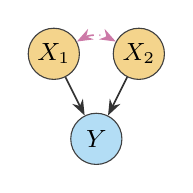
\begin{tikzpicture}[x=0.72cm,y=0.72cm]
    \node[mannode] (X1) at (0,1.15) {$X_1$};
    \node[mannode] (X2) at (1.5,1.15) {$X_2$};
    \node[tgtnode] (Y) at (0.75,-0.35) {$Y$};
    \draw[diredge] (X1) -- (Y);
    \draw[diredge] (X2) -- (Y);
    \draw[bicross] (X1) to[bend left=28] (X2);
  \end{tikzpicture}
  \caption{True graph}
  \label{fig:motivating-true}
\end{subfigure}\hfill
\begin{subfigure}[t]{0.32\linewidth}
  \centering
  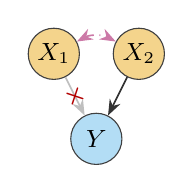
\begin{tikzpicture}[x=0.72cm,y=0.72cm]
    \node[mannode] (X1) at (0,1.15) {$X_1$};
    \node[mannode] (X2) at (1.5,1.15) {$X_2$};
    \node[tgtnode] (Y) at (0.75,-0.35) {$Y$};
    \draw[diredge,black!25] (X1) -- (Y)
      node[midway,sloped] {\textcolor{red!70!black}{\footnotesize$\boldsymbol{\times}$}};
    \draw[diredge] (X2) -- (Y);
    \draw[bicross] (X1) to[bend left=28] (X2);
  \end{tikzpicture}
  \caption{Assumed graph}
  \label{fig:motivating-assumed}
\end{subfigure}\hfill
\begin{subfigure}[t]{0.32\linewidth}
  \centering
  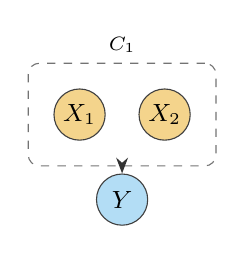
\begin{tikzpicture}[x=0.72cm,y=0.72cm]
    \node[mannode] (X1) at (0,1.15) {$X_1$};
    \node[mannode] (X2) at (1.5,1.15) {$X_2$};
    \node[tgtnode] (Y) at (0.75,-0.35) {$Y$};
    \begin{scope}[on background layer]
      \node[clbox,fit=(X1)(X2),label={[font=\scriptsize]above:$C_1$}] (C1) {};
    \end{scope}
    \draw[diredge] (C1.south) -- (Y);
  \end{tikzpicture}
  \caption{Common quotient}
  \label{fig:motivating-quotient}
\end{subfigure}

\caption{\textsc{ParallelParent}. Deleting $X_1\to Y$ changes the fine
search space but not the quotient because $C_1\to Y$ remains through
$X_2\to Y$. Orange nodes are manipulable, blue is the target, and the
dash-dotted edge denotes latent confounding.}
\label{fig:motivating}
\end{figure}

\paragraph{Why a wrong edge matters.}
Suppose $X_1$ and $X_2$ are confounded parents of $Y$, and the optimum
requires intervening on both. If the assumed graph deletes $X_1\to Y$,
fine-graph \CBO{} removes every intervention containing $X_1$. It can no
longer reach the optimum. Now group the two variables into
$C_1=\{X_1,X_2\}$. The quotient still contains $C_1\to Y$ through
$X_2\to Y$ (Fig.~\ref{fig:motivating}). Its action set therefore does not
change. This is the central trade-off: a fine graph can exclude useful
actions, while a quotient is stable but restricts intervention to whole
clusters.

\paragraph{Quotient CBO.}
We study the middle ground between trusting one full DAG and learning a DAG
online. The input is a partition $\Pi$ and a cluster DAG (C-DAG). \QCBO{}
applies \CBO{}'s arm rule to this quotient and uses identifiable cluster
effects as prior means \citep{CausalEffectIdentification}.

\paragraph{Contributions.}
\begin{itemize}[leftmargin=1.2em,itemsep=1pt,topsep=2pt]
  \item \textbf{Robustness.} One wrong edge can give a fine-graph method
  arbitrary linear regret. A quotient method is exactly invariant when the
  quotient is unchanged (Theorem~\ref{thm:separation}).
  \item \textbf{Price.} We characterize when coarsening is free, when it
  creates a linear regret floor, and how that price changes as clusters are
  split (Cor.~\ref{cor:reach}; Props.~\ref{prop:price}, \ref{prop:floor}).
  \item \textbf{Scope.} The contract applies to arm-based, dynamic, and
  model-based \CBO{}, and the experiments expose the same robustness--price
  tradeoff in all three families.
\end{itemize}

% =============================================================================
\section{Background}
\label{sec:background}

A structural causal model
$\mathcal{M}=\langle\mathbf{U},\mathbf{V},F,P(\mathbf{U})\rangle$
induces observational and interventional distributions
\citep{pearlCausality2009}. Here $\mathbf U$ are exogenous variables,
$\mathbf V$ are model variables, $F$ are their structural mechanisms, and
$P(\mathbf U)$ is the exogenous distribution. Its latent projection is an acyclic directed
mixed graph (ADMG) $\Gg=(\mathbf V,E)$ with directed causal edges and
bidirected latent-confounding edges
\citep{leeStructuralCausalBandits2019}.

\paragraph{Causal Bayesian optimization.}
Given manipulable variables $\mathbf{X}\subseteq\mathbf{V}$ and target $Y$,
an intervention arm is a nonempty set $\mathbf X_s\subseteq\mathbf X$.
\CBO{} \citep{agliettiCausalBayesianOptimization2020b} chooses an arm and
its assigned values by solving
\begin{equation}
  \label{eq:cbo_obj}
  (\mathbf{X}_s^\star,\mathbf{x}_s^\star) =
  \arg\min_{\substack{\mathbf{X}_s\in\ES\\ \mathbf{x}_s\in D(\mathbf{X}_s)}} \E\!\left[Y\mid\doo(\mathbf{X}_s=\mathbf{x}_s)\right],
\end{equation}
where $D(\mathbf{X}_s)$ is the intervention domain. \CBO{} maintains one
Gaussian process (GP) per candidate intervention set. Its exploration set
contains the graph's minimal intervention sets (MIS)
\citep{leeStructuralCausalBandits,agliettiCausalBayesianOptimization2020b}.
An intervention set is minimal when none of its variables is redundant for
$Y$ after the whole set is intervened on. Write
$\Gg_{\bar{\mathbf X}_s}$ for the graph with incoming edges to
$\mathbf X_s$ removed, and $\An(Y)$ for the ancestors of $Y$. Then
\begin{equation}
  \label{eq:mis}
  \ES(\Gg)=\left\{S\subseteq\mathbf X:
  \substack{S\ne\emptyset,\\
  S\subseteq\An(Y)\text{ in }\Gg_{\bar S}}
  \right\}=:\mathrm{MIS}(\Gg).
\end{equation}
The first line requires a nonempty subset of manipulable variables. The
second keeps it only if every intervened variable remains an ancestor of
$Y$. Otherwise that variable is redundant. Some \CBO{} implementations
further prune MIS to possibly optimal MIS (POMIS). Our quotient construction
uses MIS; released baselines retain their original arm rule.

Each GP uses a do-calculus estimate as its prior mean when the effect is
identifiable. Thus an assumed graph enters the optimizer through
\[
 \Gg\longmapsto
 \bigl(\ES(\Gg),\{m_s^\Gg\}_{s\in\ES(\Gg)}\bigr)
 \longmapsto \tau ,
\]
where $m_s^\Gg$ is the prior-mean function for arm $s$ computed under
$\Gg$, and $\tau$ is the resulting sequence of actions and observations.
A wrong graph can therefore change a prior or the arm set itself.

\paragraph{Coarsening and C-DAGs.}
\begin{definition}[Coarsening~\citep{madaleno2026a}]
\label{def:coarsening}
For a partition $\Pi$ of $\mathbf V$, let $\chi:\mathbf V\to\Pi$ map each
vertex to its cluster. Its directed quotient has
\[
 E^\Pi=\{(\chi(u),\chi(v)):(u,v)\in E,\ \chi(u)\ne\chi(v)\}.
\]
Bidirected edges are mapped in the same way. The coarsening is valid when
the directed quotient is acyclic.
\end{definition}
\[
 Q_\Pi(\Gg):=(\Pi,\Gg^\Pi).
\]
Let $\Pi_M:=\{C\in\Pi:C\subseteq\mathbf X\}$ be the manipulable clusters.
The allowed coarse interventions are all nonempty unions of these clusters:
\[
 \mathcal U(\Pi)=
 \left\{\bigcup_{C\in S}C:\emptyset\ne S\subseteq\Pi_M\right\},
\]
Thus $\mathcal U(\Pi)$ is the action family allowed by the partition. For
$A\subseteq\mathbf X$, define
\begin{align}
 \mu^\star(A)&:=\min_{a\in D(A)}\E[Y\mid\doo(A=a)],\nonumber\\
 V(\Pi)&:=\min_{A\in\mathcal U(\Pi)}\mu^\star(A),\nonumber\\
 \Delta(\Pi)&:=V(\Pi)-V(\Pi_\bot).\nonumber
\end{align}
Let $\Pi_\bot:=\{\{v\}:v\in\mathbf V\}$ be the finest partition, in which
every variable is its own cluster. It is not the partition that collapses
all variables into one cluster. Then $\mathcal U(\Pi_\bot)$ contains all
nonempty subsets of $\mathbf X$. Let $\ESpi$ be the MIS of the quotient,
expanded back to their fine variables. Lemma~\ref{lem:reduction} gives
\begin{equation}
\label{eq:value-link}
 \min_{A\in\ESpi}\mu^\star(A)
 =\min_{A\in\mathcal U(\Pi)}\mu^\star(A)=V(\Pi).
\end{equation}
C-DAG identification is sound and complete over the fine graphs represented
by the quotient \citep{CausalEffectIdentification}. Cluster-level Markov
properties transfer; faithfulness does not
\citep{wahlFoundationsCausalDiscovery2024}.

\paragraph{Evaluation metrics.}
Let $y^\star:=V(\Pi_\bot)$ and let $\hat a_t$ be the incumbent after trial
$t$. Let $\mu(\hat a_t)$ be its expected outcome. Incumbent mean regret is
\[
 r_t:=\mu(\hat a_t)-y^\star\ge0,
 \qquad R_T:=\sum_{t=1}^T r_t .
\]
The experiments also report paired trajectory differences between correct
and misspecified inputs.

% =============================================================================
\section{What coarsening buys}
\label{sec:theory}

To compare the cost of different resolutions, we compare a partition with
its refinements. A refinement splits one or more clusters. We write $\Pi'\preceq\Pi$ when
every cluster of $\Pi'$ is contained in a cluster of $\Pi$. An optimizer
satisfies the quotient contract when its graph-dependent components use
$\Gg$ only through $Q_\Pi(\Gg)$.

\begin{lemma}[Quotient contract]
\label{lem:contract}
If
\[
 \mathcal A(\Gg,\mathcal D,\omega,\eta)
 =\bar{\mathcal A}(Q_\Pi(\Gg),\mathcal D,\omega,\eta),
\]
then, for fixed data $\mathcal D$, random stream $\omega$, and
hyperparameters $\eta$,
\[
 Q_\Pi(\Gg)=Q_\Pi(\Gg')
 \quad\Longrightarrow\quad
 \tau_{\mathcal A}(\Gg)=\tau_{\mathcal A}(\Gg').
\]
\end{lemma}
This invariance follows directly from the definition. The lemma states the
contract that our methods satisfy. The main questions are what the contract
costs (\S\ref{sec:theory-price}) and what it protects against
(\S\ref{sec:theory-payoff}). Protection is defined over a class of fine
graphs:

\begin{definition}[Protected class]
\label{def:protected}
For an ADMG $\Gg$ over $\mathbf V$ and a valid partition $\Pi$,
\[
 E_\Pi(\Gg):=\{\Gg'\ \text{ADMG over}\ \mathbf V:
 Q_\Pi(\Gg')=Q_\Pi(\Gg)\}.
\]
\end{definition}
Within-cluster edits and quotient-redundant cross-cluster edits stay
inside $E_\Pi(\Gg)$ and are protected. Quotient-visible edits leave the
class and are not.

\subsection{What does protection cost?}
\label{sec:theory-price}

\begin{proposition}[Monotonicity and price of coarsening]
\label{prop:price}
For valid $\Pi'\preceq\Pi$,
\[
 \mathcal U(\Pi)\subseteq\mathcal U(\Pi'),\qquad
 0\le\Delta(\Pi')\le\Delta(\Pi).
\]
Moreover,
\[
 \Delta(\Pi)=0
 \iff
 \arg\min_{A\in\mathcal U(\Pi_\bot)}\mu^\star(A)
 \cap\mathcal U(\Pi)\ne\emptyset .
\]
\end{proposition}

\begin{proposition}[Sufficient conditions for zero coarsening gap]
\label{prop:free}
Assume a semi-Markovian SCM. For every $A\subseteq\mathbf X$, define
\begin{align*}
 \operatorname{cl}_\Pi(A)
 &:=\bigcup\{C\in\Pi:C\cap A\ne\emptyset\},\\
 B&:=\operatorname{cl}_\Pi(A)\setminus A .
\end{align*}
For each $a\in D(A)$ let $B_a$ be the joint natural response under
$\doo(A=a)$ and set
\[
 D_B(a):=\{b:(a,b)\in D(\operatorname{cl}_\Pi(A))\}.
\]
If, for all $A,a$, the \emph{support inclusion} and \emph{cross-world
independence} premises
\[
 \operatorname{supp}(B_a)\subseteq D_B(a),
 \qquad B_a\perp Y_{a,b}\quad\forall b\in D_B(a)
\]
hold, then $V(\Pi)=V(\Pi_\bot)$ and $\Delta(\Pi)=0$.
\end{proposition}

Both premises deserve names at the level a practitioner can check. The
first is a domain condition:

\begin{definition}[Full intervention support]
\label{def:fullsupport}
Intervention domains are products, $D(W)=\prod_{w\in W}D(w)$ for every
$W\subseteq\mathbf X$, and for every manipulable $v$ and every
intervention $a$ on any $A\subseteq\mathbf X\setminus\{v\}$,
$\operatorname{supp}(v_a)\subseteq D(v)$: each variable's intervention
domain contains every value it attains as a natural response.
\end{definition}

The second premise couples potential outcomes under different
interventions. We give a graph-level condition that implies
it, stated where the proof actually operates: in the augmented NPSEM
graph.

\begin{definition}[Cluster-contained confounding]
\label{def:ccc}
Represent the semi-Markovian SCM by an NPSEM with mutually independent
exogenous variables, one shared exogenous variable per bidirected edge,
and augmented graph $\Gg^{\mathrm{aug}}$. For $A\subseteq\mathbf X$
with $B=\operatorname{cl}_\Pi(A)\setminus A$, let $\mathbf U_B(A)$ be
the exogenous ancestors of $B$ in $\Gg^{\mathrm{aug}}$ mutilated by
$\doo(A)$ (the members of $B$ respond naturally and are not clamped),
and let $\mathbf U_Y(A)$ be the exogenous ancestors of $Y$ in
$\Gg^{\mathrm{aug}}$ mutilated by $\doo(\operatorname{cl}_\Pi(A))$.
The partition $\Pi$ has \emph{cluster-contained confounding} when
$\mathbf U_B(A)\cap\mathbf U_Y(A)=\emptyset$ for every
$A\subseteq\mathbf X$.
\end{definition}
Informally: once a cluster union is clamped, no latent influence is
shared between the un-clamped remainder of a cluster and the target.
A familiar sufficient ADMG condition is that every backdoor path from a
cluster member to $Y$ meets another member of that cluster before reaching
$Y$. This condition is sufficient for Def.~\ref{def:ccc}
(App.~\ref{app:proofs}); the exogenous-ancestor statement is the
condition the proof consumes.

\begin{corollary}[Graphical zero-gap condition]
\label{cor:reach}
In a semi-Markovian model, full intervention support
(Def.~\ref{def:fullsupport}) implies support inclusion, and
cluster-contained confounding (Def.~\ref{def:ccc})
implies cross-world independence (Lemma~\ref{lem:ccc}). Hence the
premises of Prop.~\ref{prop:free} hold and $\Delta(\Pi)=0$.
\end{corollary}

\begin{remark}[On the cross-world premise]
\label{rem:crossworld}
$B_a\perp Y_{a,b}$ is untestable from any single-world data,
observational or from any one experiment. Cor.~\ref{cor:reach}
therefore never invokes it as a primitive: within an NPSEM
representation with mutually independent exogenous variables it is
\emph{derived}, via Lemma~\ref{lem:ccc}, from Def.~\ref{def:ccc},
an ordinary structural judgement about where confounding lives. The
premise inherits exactly the credibility of that judgement, no more.
\end{remark}

Within this model class, the contrapositive is
\[
 \Delta(\Pi)>0\Longrightarrow
 \substack{\text{support failure or}\\
 \text{confounding escaping a cluster}.}
\]
Thus coarsening need not sacrifice the best attainable value. Even when
$\Delta(\Pi)=0$, it may change finite-sample regret, dimension, and
intervention cost.

\subsection{What protection buys: worst-case regret}
\label{sec:theory-payoff}

Fix a true SCM $\mathcal M$ with latent projection $\Gg$, and hand the
optimizer a \emph{hypothesis} graph $H$ while every intervention
outcome is drawn from $\mathcal M$ (the fixed-objective seam of
\S\ref{sec:exp}; App.~\ref{app:seam}). Write $R_T(\mathcal A;H)$ for
the incumbent regret of \S\ref{sec:background} when $\mathcal A$ runs
with input $H$ at fixed $(\mathcal D,\omega,\eta)$, and
\[
 \mathrm{WR}_T(\mathcal A):=\sup_{H\in E_\Pi(\Gg)}R_T(\mathcal A;H)
\]
for the worst case over the protected class.

\begin{theorem}[Protected-class regret separation]
\label{thm:separation}
\begin{enumerate}[label=(\roman*),leftmargin=1.6em,itemsep=1pt,topsep=2pt]
\item \textbf{Fine-graph fragility.} For every $\beta>0$ there exist a
semi-Markovian SCM $\mathcal M_\beta$ (\textsc{ParallelParent} with its
curvature chosen to give gap $\beta$, App.~\ref{app:minibench}), a valid $\Pi$ with
$\Delta(\Pi)=0$, and $H\in E_\Pi(\Gg)$ obtained from $\Gg$ by deleting
a single directed edge, such that every optimizer whose initial and
sequential intervention sets all lie in
$\mathrm{MIS}(H)$, and whose incumbent is selected among those executed
interventions, satisfies $r_t\ge \beta$ for all $t$, hence
$\mathrm{WR}_T\ge \beta T$.
\item \textbf{Uniform protection with exact decomposition.} For every
$\mathcal M$, valid $\Pi$, and fixed $(\mathcal D,\omega,\eta)$: if
$\mathcal A$ satisfies the quotient contract for $\Pi$, executes only
interventions on cluster unions $A\in\mathcal U(\Pi)$, and selects its
incumbent among executed actions, then its trajectory is identical for
every $H\in E_\Pi(\Gg)$ and
\[
\begin{aligned}
 \mathrm{WR}_T(\mathcal A)&=R_T(\mathcal A;\Gg)\\
 &=T\,\Delta(\Pi)
 +\sum_{t=1}^T\bigl(\mu(\hat a_t)-V(\Pi)\bigr),
\end{aligned}
\]
with both terms nonnegative: an unavoidable per-trial structural gap,
plus within-quotient optimization regret that no member of the
protected class can alter.
\end{enumerate}
\end{theorem}

Part (i) is the headline: a single quotient-invisible edge deletion
costs a fine-graph method an arbitrarily large linear regret while the
quotient loses nothing ($\Delta(\Pi)=0$). Experiment~A instantiates the
construction at $\lambda=1$ (\S\ref{sec:exp-a}). Part (ii) prices the
protection exactly. A converse closes the design space:

\begin{proposition}[The contract is necessary for trajectory-level
protection]
\label{prop:converse}
If the trajectory map $H\mapsto\tau(H)$ at fixed
$(\mathcal D,\omega,\eta)$ is constant on $E_\Pi(\Gg)$ for every ADMG
$\Gg$, then it factors through $Q_\Pi$.
\end{proposition}
This characterizes the \emph{trajectory map}, not an optimizer's
internal implementation: any procedure whose behavior is invariant
over every protected class is, at the trajectory level, a function of
the quotient alone.

\paragraph{Refining the partition: Hierarchical \QCBO{} (\HQCBO{}).}
\label{sec:refine}
\begin{proposition}[Linear regret floor under a fixed partition]
\label{prop:floor}
For a fixed partition,
\[
 r_t\ge\Delta(\Pi)\ \text{ for every }t,\qquad R_T\ge T\Delta(\Pi).
\]
\end{proposition}
The floor concerns the incumbent mean, not the exploratory action at
trial $t$: a positive action-space gap contributes linearly in the
horizon, and no within-quotient learning removes it. Refinement can.
\HQCBO{} starts at $\Pi$ and splits the incumbent's clusters along a
declared hierarchy when progress stalls; it rejects refinements whose
quotient is cyclic, retains old-arm data, and initializes only new arms.
Appendix~\ref{app:proofs} gives the technical refinement properties.

\begin{definition}[Incumbent consistency]
\label{def:consistency}
The base optimizer's incumbent is \emph{consistent} on the action
space of a partition $\Pi_J$ if, when the optimizer continues on that
action space, $\mu(\hat a_t)\to V(\Pi_J)$ almost surely as
$t\to\infty$.
\end{definition}

\begin{corollary}[Conditional refinement recovery]
\label{cor:recovery}
If the refinement schedule visits a valid $\Pi_J$ with
$\Delta(\Pi_J)=0$ and the incumbent is consistent on $\Pi_J$'s action
space (Def.~\ref{def:consistency}), then $r_t\to0$ and $R_T/T\to0$.
\end{corollary}
Whether $\Pi_J$ is visited depends on the trigger, a \emph{heuristic}
with no guarantee: \HQCBO{} splits when the best-so-far value has
improved by less than $\delta$ over the last $k$ trials (exact rule
and defaults in App.~\ref{app:seam}). Cor.~\ref{cor:recovery} is
conditional on the trigger firing, on the declared hierarchy exposing
an optimal arm, and on consistency of the base optimizer. We assume
consistency rather than prove it. With continuous within-arm domains and
unbounded noise it fails for, e.g., raw running minima of noisy
observations.

\begin{corollary}[Adaptive refinement invariance]
\label{cor:adaptive_invariance}
Write $\tau_{\mathcal H}$ for the \HQCBO{} trajectory under a
declared hierarchy $\mathcal H$. For visited partitions
$\Pi_0,\ldots,\Pi_J$,
\[
 \left[\forall j,\ \Gg^{\Pi_j}=(\Gg')^{\Pi_j}\right]
 \Longrightarrow \tau_{\mathcal H}(\Gg)=\tau_{\mathcal H}(\Gg').
\]
\end{corollary}
Splitting a cluster exposes its internal edges in later phases. Edits inside
clusters that are never split remain invisible.

% =============================================================================
\section{Instantiations: \QCBO{}, \QDCBO{}, and \QMCBO{}}
\label{sec:method}

Each variant replaces only the base method's graph-dependent components.
Appendix~\ref{app:seam} gives implementation details.

\subsection{Arm-based: quotient \CBO{} (\QCBO{})}
\label{sec:setup}
\QCBO{} receives a manipulable partition and its C-DAG; all other variables
remain singletons. With $U_\Pi(S):=\bigcup_{C\in S}C$, its arms are
\begin{equation}
  \label{eq:ccbo_exploration}
 \ESpi=\left\{U_\Pi(S):
 \begin{array}{l}
 \emptyset\ne S\subseteq\Pi_M,\\[-2pt]
 S\subseteq\An(Y)\text{ in }\Gq_{\bar S}
 \end{array}\right\}.
\end{equation}
Thus every arm sets complete clusters.

\paragraph{Identifiability and the two-tier prior.}
\label{sec:causal_prior}
For each arm, complete ID determines whether the observational data identify
its prior mean \citep{shpitserIdentificationJointInterventional,AnankeModuleCausal}:
\begin{equation}
  \label{eq:two_tier_prior}
  m_A(a) = \begin{cases}
    \hat{\E}[Y\mid\doo(A=a)]
      & \text{if identified in }\Gq,\\
    \bar{Y}_{\mathrm{obs}} & \text{otherwise.}
  \end{cases}
\end{equation}
Non-identifiable arms start at the observational mean and learn from trials.
C-DAG identification is sound for every represented fine graph
\citep{CausalEffectIdentification}.

\begin{assumption}[Estimator boundary]
\label{ass:valid}
The quotient is valid. The ID test is complete, while our numerical
estimator is sound but not complete. Identifiable expressions outside its
implemented class receive the uninformative prior.
\end{assumption}

\begin{proposition}[Identity recovery]
\label{prop:identity}
\begin{align*}
 \Pi=\Pi_\bot\Longrightarrow\quad
 \Gg^\Pi&=\Gg^\star,\\
 \ESpi&=\mathrm{MIS}(\Gg^\star),&
 m_A^\Pi&=m_A^{\CBO}.
\end{align*}
\end{proposition}
This matches \CBO{} as specified; App.~\ref{app:seam} documents two corrected
implementation deviations.

\subsection{Dynamic: quotient DCBO (\QDCBO{})}
\label{sec:qdcbo}
\QDCBO{} quotients each dynamic-network slice and its transitions, then uses
joint cluster mechanisms and Eq.~\eqref{eq:ccbo_exploration} per slice
\citep{agliettiDynamicCausalBayesian2021a}.

\begin{corollary}[\QDCBO{} inherits the contract]
\label{cor:qdcbo_invariance}
\QDCBO{} satisfies Lemma~\ref{lem:contract} per slice. At
$\Pi=\Pi_\bot$ it equals DCBO, and Prop.~\ref{prop:price} applies to each
slice's reachable interventions.
\end{corollary}

\subsection{Model-based: quotient MCBO (\QMCBO{})}
\label{sec:qmcbo}
MCBO composes GP mechanisms and optimizes with GP-UCB
\citep{srinivasGaussianProcessOptimization2010,sussexMODELBASEDCAUSALBAYESIAN2023}.
\QMCBO{} replaces node mechanisms by
\[
 P(\mathbf X_C\mid\mathbf X_{\mathrm{pa}(C)}),
\]
multi-output GPs composed along the C-DAG
\citep{bonillaMultitaskGaussianProcess2007}.

\begin{corollary}[\QMCBO{} inherits the contract]
\label{cor:qmcbo_invariance}
\QMCBO{} satisfies Lemma~\ref{lem:contract}. At $\Pi=\Pi_\bot$ it equals
MCBO. Its reachable interventions are whole-cluster patterns, so
Prop.~\ref{prop:price} also applies.
\end{corollary}

\begin{proposition}[Soundness of cluster mechanisms]
\label{prop:qsound}
Under causal sufficiency and valid $\Pi$, for every union of clusters $S$,
\[
 P(\mathbf V\mid\doo(\mathbf x_S))
 =\prod_{C\notin S}
 P(\mathbf X_C\mid\mathbf X_{\mathrm{pa}(C)})
 \big|_{\mathbf X_S=\mathbf x_S}.
\]
The mechanism must be joint to retain within-cluster dependence.
\end{proposition}

\begin{proposition}[Exposure: sub-cluster interventions are not identifiable
from cluster mechanisms]
\label{prop:qexposure}
There exist causally sufficient SCMs $M_1,M_2$, valid for the same $\Pi$,
such that
\begin{align*}
 \mathcal I_\Pi(M_1)&=\mathcal I_\Pi(M_2),\\
 P^{M_1}(Y\mid\doo(x_A))
 &\ne P^{M_2}(Y\mid\doo(x_A))
\end{align*}
for a strict subset $A\subsetneq C$. Here $\mathcal I_\Pi$ contains the
joint cluster mechanisms and all whole-cluster interventional
distributions.
\end{proposition}

\paragraph{Input.}
The method needs a partition and C-DAG, not a fine graph. Clusters can follow
known modules or a domain taxonomy. Validity is an acyclicity check and must
be repeated after refinement. Some restricted model classes also permit
statistical tests of a proposed coarsening
\citep{madalenoCoarseningLinearNonGaussian2026}.
% TODO(extension): develop data-driven partition and hierarchy selection.

% =============================================================================
\section{Experiments}
\label{sec:exp}

We first isolate quotient invariance, prior corruption, and the action-space
gap on three SCMs with closed-form oracles. We then test all three optimizer
families on their standard benchmarks. Full specifications are in
App.~\ref{app:minibench}.

\paragraph{Protocol.}
Only the assumed structure changes. The minimal suite uses $30$ paired seeds,
$n_{\mathrm{obs}}=100$, $T=50$ ($60$ for \textsc{MediatedChain}), three
initial points per arm, and unit cost per intervened variable. We report
best-so-far values and paired trajectory differences. Appendix~\ref{app:repro}
specifies initialization, matched budgets, estimators, and refinement.

\begin{table*}[t]\centering
  \caption{By Lemma~\ref{lem:contract}, rows with an unchanged quotient
  are predicted invariant. The final column reports the measured paired
  deviation. PP = \textsc{ParallelParent}, FD = \textsc{FrontDoor}.}
  \label{tab:minimal-taxonomy}
  \adjustbox{max width=\linewidth}{\begin{tabular}{llcccc}
\hline
Condition & Edit & Quotient & Fine MIS & Fine prior & Role\\
 & & changed & changed & changed & \\
\hline
A1 (PP) & delete $X_1\to Y$ & no & yes & -- & primary\\
A2 (PP) & add $X_1\to X_2$ & no & no & yes & diagnostic\\
A3 (PP) & add $X_1\leftrightarrow Y$ & yes & no & yes & diagnostic\\
B1 (FD) & add $X_1\leftrightarrow M$ & no & no & yes & primary\\
\hline
\end{tabular}
}
\end{table*}

\subsection{Experiment A: exploration-set corruption}
\label{sec:exp-a}
\textsc{ParallelParent} uses the SCM from Fig.~\ref{fig:motivating} with
$\lambda=1$. The fine MIS is
$\{\{X_1\},\{X_2\},\{X_1,X_2\}\}$ and $y^\star=0$. Deleting
$X_1\to Y$ leaves only $\{X_2\}$, whose population optimum is $4.25$.
Fine \CBO{} ends at mean $4.245$ on the deterministic $100{,}000$-draw
common-random-number objective (Fig.~\ref{fig:minimal-misspec}a). The small
difference reflects Monte Carlo and finite-budget optimization error. This instantiates
Theorem~\ref{thm:separation}(i) at $\lambda=1$.
For $\Pi=\{\{X_1,X_2\}\}$ the deletion is quotient-invisible, and every
\QCBO{} trajectory is identical under the two graphs
($\sup|\Delta|=0$). A spurious $X_1\leftrightarrow Y$ is a
quotient-visible negative control and changes the \QCBO{} trajectory.

\begin{figure*}[t]\centering
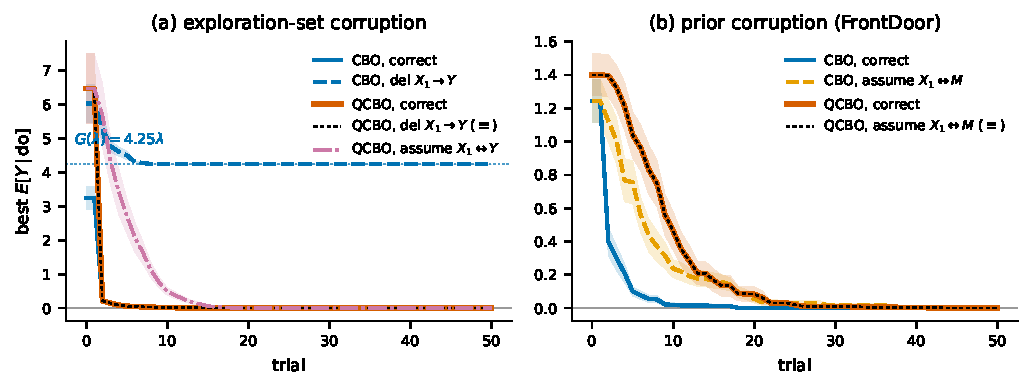
\includegraphics[width=\textwidth]{figures/minimal_misspec}
\caption{Correct and misspecified trajectories, mean$\pm$s.e.\ over $30$
seeds. (a) A wrong fine graph removes the optimal arm, while \QCBO{} is
unchanged for the quotient-invisible edit. (b) Prior corruption slows fine
\CBO{} transiently, while \QCBO{} remains exactly invariant.}
\label{fig:minimal-misspec}
\end{figure*}

\subsection{Experiment B: prior corruption without arm loss}
\label{sec:exp-b}
\textsc{FrontDoor} uses $X_1\to M\to Y$, latent
$X_1\leftrightarrow Y$, and a narrow-well objective whose optimum is
$\doo(M=1)$. Adding a spurious $X_1\leftrightarrow M$ preserves the fine
MIS but removes its identified priors. Fine \CBO{} pays an empirical
$\Delta R_{50}=6.1\pm1.0$ and then reaches a similar final value
($0.006$ versus $0.001$). Under $\Pi=\{\{X_1,M\}\}$ the edit is internal.
\QCBO{} is identical across conditions ($\sup|\Delta|=0$).

\subsection{Experiment C: the price of coarsening, and buying it back}
\label{sec:exp-c}
\textsc{MediatedChain} has $X_1\to X_2\to Y$,
$X_2=2X_1+\varepsilon_2$, $Y=(X_2-4)^2$, and
$D(X_2)=[-2,2]$. For $\Pi=\{\{X_1,X_2\}\}$,
\[
 V(\Pi)=4,\qquad y^\star=0.04,\qquad\Delta(\Pi)=3.96.
\]
The support condition in Prop.~\ref{prop:free} fails because
$\doo(X_1=2)$ lets $X_2$ respond near $4$, outside its intervention box.
\CBO{}, \QCBO{}, and \HQCBO{} finish at $0.040$, $4.000$, and $0.040$.
\HQCBO{} refines at trial $7.5\pm0.1$. The fixed-partition empirical
regret tracks the floor of Prop.~\ref{prop:floor}, while the refined
curve flattens after the fine arm appears:
$R_{60}=5.60\pm1.69$ (\CBO{}), $243.23\pm0.91$ (\QCBO{}, against the
floor $T\Delta(\Pi)=237.6$), and $37.22\pm1.21$ (\HQCBO{}).

\begin{figure}[t]\centering
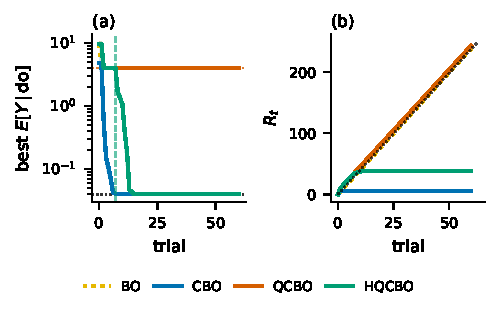
\includegraphics[width=\linewidth]{figures/minimal_refine}
\caption{\textsc{MediatedChain} over $30$ seeds. Top: mean$\pm$s.e.\
best-so-far value and mean refinement time. Bottom: mean empirical cumulative
regret, excluding the shared initial incumbent. Refinement exposes the fine
optimal arm.}
\label{fig:minimal-refine}
\end{figure}

\subsection{Experiment D: portability across families}
\label{sec:exp-d}
We compare each quotient method with its base in the base paper's released
stack and metric. The suite contains three \CBO{} tasks ($10$ seeds), three
DCBO tasks ($20$ seeds), and two MCBO tasks ($20$ seeds). Graphs and full
protocols are in Apps.~\ref{app:dags} and~\ref{app:repro}.

\textbf{Results.}
The structural result is exact: \QDCBO{} is invariant in all $60$ paired
dynamic runs, and \QMCBO{} in all $40$ paired model-based runs. Their base
methods change. Finite-budget performance is mixed, as expected from
$\Delta(\Pi)$. Quotient variants improve the two stationary dynamic tasks
and MCBO ToyGraph, lose on Synthetic and Coral, and tie on the remaining
tasks (App.~\ref{app:fulltables}). With matched initialization budgets, the
Synthetic loss disappears; on Coral, the base method cannot finish its
$31$-arm initial design within the quotient method's total budget
(App.~\ref{app:repro}).

\paragraph{Graph-uncertain comparator (\CEO{}).}
\CEO{} learns over observable DAGs online
\citep{branchiniCausalEntropyOptimization2023}. It improves robustness to
A1: $0.77$ versus committed \CBO{}'s $4.245$. Yet \QCBO{} is exactly
invariant and better by $0.07$--$1.00$ on every protected condition.
\CEO{} cannot represent the latent-confounder errors A3/B1. Conversely, its
fine action space avoids the fixed quotient's price in
\textsc{MediatedChain} ($0.135$ versus $4.000$), while \HQCBO{} reaches
$0.040$. Thus graph learning and quotient commitment protect against
different errors. Table~\ref{tab:ceo} and App.~\ref{app:repro} give the full
protocol and cost accounting.

% =============================================================================
\section{Related work}
\label{sec:related}

\paragraph{Structural uncertainty.}
GACBO and \CEO{} learn over DAGs online
\citep{mukherjeeGraphAgnosticCausal2024,branchiniCausalEntropyOptimization2023};
other work learns $\Pa(Y)$ or a MAG under additional assumptions
\citep{durandCausalBayesianOptimization2025,parkStructuralCausalBandits}.
Causal-bandit guarantees likewise price learning an unknown graph inside the
horizon \citep{luCausalBanditsUnknown2021,konobeevCausalBanditsGraph2025,
maitiCausalBanditApproach2022}. We instead price commitment to a fixed
coarse input. These approaches are complementary: an online learner could
operate over, or refine, a quotient.

\paragraph{Identification and abstraction.}
C-DAG identification is sound and complete
\citep{CausalEffectIdentification}; we build an optimization contract on
that layer. Coarsening also connects to causal abstraction and macro-level
structure learning
\citep{beckersAbstractingCausalModels2019,madaleno2026a,
ferreiraIdentifyingMacroCausal2025}. Unlike outcome coarsening
\citep{zeitlerMFACBOMultiFidelityAbstraction2025}, we coarsen manipulable
inputs. Faithfulness need not survive this operation
\citep{wahlFoundationsCausalDiscovery2024}.

% =============================================================================
\section{Discussion and limitations}
\label{sec:limitations}
Protection requires the correct quotient. Quotient-visible errors and wrong
partitions remain harmful. The zero-gap condition is structural and its
cross-world consequence is not testable from single-world data. Refinement
is heuristic; Cor.~\ref{cor:recovery} is conditional. Initialization costs
differ when arm counts differ, so App.~\ref{app:repro} also reports matched
total budgets. Computing the arm set needs up to $2^K-1$ MIS and ID checks
for $K$ manipulable clusters. \QMCBO{}, like MCBO, assumes causal
sufficiency.
% TODO(extension): evaluate learned partitions, GACBO, random graph errors,
% and the cost of unnecessary refinement.
% TODO(extension): derive testable zero-gap conditions or sensitivity bounds,
% and conditions under which refinement exposes an optimal fine arm.

% =============================================================================
\section{Conclusion}
\label{sec:conclusion}
A quotient protects exactly what it preserves. Within that class, its
trajectory cannot change. Outside it, protection has an explicit action-space
price. The separation theorem and experiments show both sides: coarsening can
prevent catastrophic graph errors, but only refinement can recover actions
that the quotient removes.

\bibliographystyle{abbrvnat}
\bibliography{references}

% =============================================================================
\appendix
\onecolumn

\section{Proofs}\label{app:proofs}
Notation is as in \S\ref{sec:setup} and \S\ref{sec:theory}.

\begin{proof}[Proof of Lemma~\ref{lem:contract}]
Write the run as decisions $d_1,d_2,\ldots$ and datasets
$\mathcal D_0,\mathcal D_1,\ldots$, with
\[
d_t=f_t\!\left(Q_\Pi(\Gg),\mathcal D_{t-1},\omega_t,\eta\right).
\]
When $Q_\Pi(\Gg)=Q_\Pi(\Gg')$, the first arguments agree. The fixed-objective
protocol also fixes $\mathcal D_0$, the random stream, and the
hyperparameters. Thus $d_1$ and the resulting $\mathcal D_1$ agree.
Induction gives equality of every decision, dataset, and stopping event, hence
of the full trajectories. Within-cluster edits and cross-cluster edits
redundant in the quotient leave $Q_\Pi(\Gg)$ unchanged, which proves the
stated scope.
\end{proof}

\begin{lemma}[MIS reduction]
\label{lem:reduction}
Let $G$ be an ADMG with manipulable vertices $M$ and target $Y$, let
$\emptyset\neq\mathbf{W}\subseteq M$, and set
$\mathbf{W}' = \mathbf{W}\cap \An(Y)$ computed in $G_{\bar{\mathbf{W}}}$.
Then (i) $P(Y\mid\doo(\mathbf{W}=\mathbf{w})) =
P(Y\mid\doo(\mathbf{W}'=\mathbf{w}|_{\mathbf{W}'}))$ for every $\mathbf{w}$,
(ii) $\mathbf{W}'$ is a MIS (or empty, when no member reaches $Y$), and
(iii) consequently
$\min_{\mathbf{X}_s\in\mathrm{MIS}(G)}\mu^\star(\mathbf{X}_s)
 = \min_{\emptyset\neq\mathbf{W}\subseteq M}\mu^\star(\mathbf{W})$:
restricting the search to MIS loses no value.
\end{lemma}

\begin{proof}
(i) In $G_{\bar{\mathbf{W}}}$ the members of
$\mathbf{W}\setminus\mathbf{W}'$ have no directed path to $Y$, so $Y$ is
unaffected by their values under the intervention. Dropping them from the
intervention changes no mechanism on any directed path into $Y$
(do-calculus rule 3). (ii) A directed path from $w'\in\mathbf{W}'$ to $Y$
in $G_{\bar{\mathbf{W}}}$ passes through no intervened vertex (their
incoming edges are cut), hence through no member of
$\mathbf{W}\supseteq\mathbf{W}'$. The same path exists in
$G_{\bar{\mathbf{W}}'}$, which only restores edges, so
$\mathbf{W}'\subseteq\An(Y)$ there. (iii) By (i) and (ii) every candidate's
value is attained by a MIS, and $\mathrm{MIS}(G)$ is a subset of the
candidates.
\end{proof}

\paragraph{Technical refinement facts.}
\begin{proposition}[A refinement can invalidate a quotient]
\label{prop:refinement_validity}
There exist a valid partition $\Pi$ and a refinement $\Pi'\preceq\Pi$ for
which $\Gg^\Pi$ is acyclic but $\Gg^{\Pi'}$ contains a directed cycle.
Validity must therefore be checked after every split.
\end{proposition}

\begin{proposition}[Retained arms after refinement]
\label{prop:refinement}
Let $\Pi'\preceq\Pi$ be valid. If
$A\in\ES^\Pi\cap\mathrm{MIS}(\Gg^{\Pi'})$, then $A\in\ES^{\Pi'}$.
If $P(Y\mid\doo(A))$ is identified from $\Gg^\Pi$ by a functional
$\phi_A(P)$, the same functional remains valid under $\Gg^{\Pi'}$.
MIS membership itself need not be preserved.
\end{proposition}

\begin{proof}[Proof of Prop.~\ref{prop:refinement_validity}]
Take $\mathbf{X}=\{a_1,a_2,b_1,b_2\}$ with fine edges $a_1\to b_1$ and $b_2\to a_2$.
The coarsest partition $\Pi=\{\{a_1,a_2,b_1,b_2\}\}$ is valid: both edges are
intra-cluster, so the quotient has a single manipulable node and is acyclic. Its
refinement $\Pi'=\{\{a_1,a_2\},\{b_1,b_2\}\}$ exposes both edges as inter-cluster
($a_1\to b_1$ contributes $A\to B$ and $b_2\to a_2$ contributes $B\to A$), inducing
the 2-cycle $A\rightleftarrows B$, so $\mathcal{G}^{\Pi'}$ is cyclic and $\Pi'$ is
invalid. Decidability is immediate from the acyclicity clause of
Def.~\ref{def:coarsening}.
\end{proof}

\begin{proof}[Proof of Prop.~\ref{prop:refinement}]
(i) Membership at $\Pi'$ is the stated hypothesis (any union of
$\Pi$-clusters is a union of $\Pi'$-clusters, so the candidate exists at
$\Pi'$, and being a MIS of $\Gg^{\Pi'}$ puts it in $\ES^{\Pi'}$). For the
identification functional, quotienting is compositional. The graph $\Gq$ is
the quotient of $\mathcal{G}^{\Pi'}$ under the induced partition of
$\Pi'$-clusters, so every fine graph compatible with $\mathcal{G}^{\Pi'}$
is compatible with $\Gq$. Identifiability from $\Gq$ means a single
functional of the observational distribution equals
$\E[Y\mid\doo(\mathbf{X}_s)]$ across all SCMs whose graph is compatible with
$\Gq$ \citep{CausalEffectIdentification}. A fortiori the same functional
works across the smaller class compatible with $\mathcal{G}^{\Pi'}$.
MIS membership can fail after refinement because restoring distinctions
between cluster members may make one member redundant under intervention.
\end{proof}

\begin{proof}[Proof of Prop.~\ref{prop:price}]
By Lemma~\ref{lem:reduction}(iii) applied to $\Gq$,
$V(\Pi)=\min_{\mathbf{X}_s\in\ESpi}\mu^\star(\mathbf{X}_s)$ equals the
minimum of $\mu^\star$ over \emph{all} non-empty unions of $\Pi$-clusters
(the value $\mu^\star$ of a cluster union is a property of the underlying
SCM, the same at every partition that can express the union). Unions of
$\Pi$-clusters are unions of $\Pi'$-clusters and, at $\Pi_\bot$, all
non-empty subsets of $\mathbf{X}$, so the three minima are over nested
candidate families: $V(\Pi_\bot)\le V(\Pi')\le V(\Pi)$. Equality
$V(\Pi)=V(\Pi_\bot)$ holds iff the unrestricted minimum is attained by a
union of $\Pi$-clusters, and by Lemma~\ref{lem:reduction}(iii) at
$\Pi_\bot$ the unrestricted minimum is $\min$ over Eq.~\eqref{eq:cbo_obj}'s
exploration set. This is exactly the stated condition.
\end{proof}

\begin{proof}[Proof of Prop.~\ref{prop:free}]
Fix $A$ and $a$. Consistency and the assumed cross-world independence give
\[
\begin{aligned}
 \E[Y_a]
 &=\int \E[Y_{a,b}\mid B_a=b]\,dP(B_a=b)\\
 &=\int \E[Y_{a,b}]\,dP(B_a=b)\\
 &\ge \inf_{b\in D_B(a)}\E[Y_{a,b}],
\end{aligned}
\]
where the support inclusion justifies the last line. Therefore
\[
 \mu^\star(\operatorname{cl}_\Pi(A))\le \mu^\star(A).
\]
The closure of every fine arm is a union of clusters, so
$V(\Pi)\le V(\Pi_\bot)$. Conversely,
$\mathcal U(\Pi)\subseteq\mathcal U(\Pi_\bot)$ implies
$V(\Pi)\ge V(\Pi_\bot)$. Hence equality holds.
\end{proof}

\begin{lemma}[Cluster containment implies cross-world independence]
\label{lem:ccc}
In an NPSEM with mutually independent exogenous variables and
augmented graph $\Gg^{\mathrm{aug}}$: if $\Pi$ has cluster-contained
confounding (Def.~\ref{def:ccc}), then for every $A\subseteq\mathbf X$,
every $a\in D(A)$, and every $b\in D_B(a)$, $B_a\perp Y_{a,b}$.
\end{lemma}

\begin{proof}
Under $\doo(A=a)$ the members of $B$ retain their mechanisms, so
recursive substitution in the mutilated model writes $B_a$ as a
measurable function of the exogenous ancestors of $B$ in
$\Gg^{\mathrm{aug}}_{\overline A}$. These are $\mathbf U_B(A)$, and the
clamped values $a$ enter as constants. Under
$\doo(\operatorname{cl}_\Pi(A)=(a,b))$, recursive substitution writes
$Y_{a,b}$ as a measurable function of $\mathbf U_Y(A)$, the exogenous
ancestors of $Y$ in
$\Gg^{\mathrm{aug}}_{\overline{\operatorname{cl}_\Pi(A)}}$. The two
ancestor sets are disjoint by Def.~\ref{def:ccc}, and the exogenous
variables are mutually independent, so any function of the first is
independent of any function of the second.
\end{proof}

\begin{proof}[Proof of Cor.~\ref{cor:reach}]
Under Def.~\ref{def:fullsupport}, the joint support of $B_a$ lies in
the product of its marginal supports, each contained in the
corresponding $D(v)$, whose product is $D_B(a)$; hence
$\operatorname{supp}(B_a)\subseteq D_B(a)$.
Lemma~\ref{lem:ccc} gives $B_a\perp Y_{a,b}$, so
Prop.~\ref{prop:free} applies.

For the ADMG reading quoted after Def.~\ref{def:ccc}: suppose some
$U^\star\in\mathbf U_B(A)\cap\mathbf U_Y(A)$. Then $U^\star$ has a
directed path $p_1$ to a member of $B$ avoiding the clamped $A$, and a
directed path $p_2$ to $Y$ avoiding the entire clamped closure. Let
$W$ be the closure member on $p_1$ nearest $U^\star$; the segment of
$p_1$ from $W$ back to $U^\star$ meets no other closure member.
Splicing it with $p_2$ at $U^\star$ yields a backdoor path from the
cluster member $W$ to $Y$ whose interior avoids every other member of
$W$'s cluster. This violates the backdoor condition. Hence that condition
phrasing implies the exogenous-ancestor disjointness of
Def.~\ref{def:ccc}: checking it in the ADMG suffices.

Both premises can be necessary. In \textsc{MediatedChain}, setting
$X_1=2$ lets the natural response of $X_2$ reach $4$, while hard
interventions constrain $X_2$ to $[-2,2]$. The support condition fails and
$\Delta(\Pi)=3.96$. For an independence counterexample, let
$C=\{A,B\}$, $B=U$, and $Y=-BU+(A-1)^2$ with $U\sim\mathcal N(0,1)$.
Then $\E[Y\mid\doo(A=1)]=-1$, whereas
$\E[Y\mid\doo(A=a,B=b)]=(a-1)^2\ge0$. Whole-cluster intervention severs
the useful dependence, giving $\Delta(\Pi)=1$ despite unrestricted domains.
\end{proof}

\begin{proof}[Proof of Theorem~\ref{thm:separation}]
(i) Let $\mathcal M_\lambda$ be \textsc{ParallelParent}
(App.~\ref{app:minibench}) with curvature $\lambda=\beta/4.25$: manipulable
$\mathbf X=\{X_1,X_2\}$, edges $X_1\to Y$ and $X_2\to Y$, latent
$X_1\leftrightarrow X_2$, domains $[-3,3]^2$, and
$\Pi=\{\{X_1,X_2\},\{Y\}\}$. Let $H$ delete $X_1\to Y$. The quotient is
unchanged because the cluster edge $C_1\to Y$ survives through $X_2\to Y$
and $X_1\leftrightarrow X_2$ is intra-cluster. Thus $H\in E_\Pi(\Gg)$, and
$\Delta(\Pi)=0$ because $\mathcal U(\Pi)=\{\{X_1,X_2\}\}$ and the joint
arm attains $y^\star=0$ at $(2,-2)\in[-3,3]^2$. In $H$, however, $X_1$
has no directed path to $Y$, so $X_1\notin\An(Y)$ in every mutilation
and Eq.~\eqref{eq:mis} gives $\mathrm{MIS}(H)=\{\{X_2\}\}$. By the
closed form of App.~\ref{app:minibench},
$\E[Y\mid\doo(X_2=x_2)]=4.25\lambda+(x_2+2)^2\ge4.25\lambda=\beta$ for
every $x_2$. Every executed intervention, including the initial design, is
an $\{X_2\}$-intervention, so every candidate incumbent satisfies
$\mu(\hat a_t)\ge \beta$, i.e.\ $r_t\ge \beta$ and $R_T(\cdot\,;H)\ge \beta T$. The
supremum over $E_\Pi(\Gg)$ is at least this value. Both restrictions
are necessary: an initial evaluation of the joint arm
$\{X_1,X_2\}\notin\mathrm{MIS}(H)$, or an incumbent chosen outside the
executed set, could otherwise seed a zero-regret incumbent.

(ii) Trajectory identity across $E_\Pi(\Gg)$ is
Lemma~\ref{lem:contract}: decisions and outcomes (drawn from the fixed
$\mathcal M$) coincide step by step, so
$R_T(\mathcal A;H)=R_T(\mathcal A;\Gg)$ for every $H\in E_\Pi(\Gg)$ and
the supremum is attained everywhere. For the decomposition, add and
subtract $V(\Pi)$ in each term of $R_T=\sum_t(\mu(\hat a_t)-y^\star)$:
\[
 r_t=\underbrace{V(\Pi)-y^\star}_{=\,\Delta(\Pi)}
 +\bigl(\mu(\hat a_t)-V(\Pi)\bigr).
\]
The incumbent is an executed action on some $A\in\mathcal U(\Pi)$, and
$V(\Pi)$ is the minimum of $\mu^\star$ over $\mathcal U(\Pi)$
(Eq.~\eqref{eq:value-link}), so $\mu(\hat a_t)\ge V(\Pi)$;
$\Delta(\Pi)\ge0$ by Prop.~\ref{prop:price}.
\end{proof}

\begin{proof}[Proof of Prop.~\ref{prop:converse}]
Constancy on $E_\Pi(\Gg)$ for every $\Gg$ means $\tau(H)$ depends
on $H$ only through the fiber of $Q_\Pi$ containing it. Setting
$\bar\tau(q):=\tau(H)$ for any $H$ with $Q_\Pi(H)=q$ is therefore well
defined, and $\tau=\bar\tau\circ Q_\Pi$.
\end{proof}

\begin{proof}[Proof of Prop.~\ref{prop:floor}]
By Lemma~\ref{lem:reduction}(iii),
$y^\star=V(\Pi_\bot)$. A fixed partition executes only arms in
$\mathcal U(\Pi)$, so every incumbent satisfies
\[
 r_t=\mu(\hat a_t)-y^\star
 \ge V(\Pi)-V(\Pi_\bot)=\Delta(\Pi).
\]
Summation gives $R_T\ge T\Delta(\Pi)$.
\end{proof}

\begin{proof}[Proof of Cor.~\ref{cor:recovery}]
A visited $\Pi_J$ with $\Delta(\Pi_J)=0$ has an exploration set
containing an optimal arm (Prop.~\ref{prop:price} and
Eq.~\eqref{eq:value-link}). Consistency in the sense of
Def.~\ref{def:consistency} gives
$\mu(\hat a_t)\to V(\Pi_J)=y^\star$ almost surely, i.e.\ $r_t\to0$,
and Ces\`aro averaging gives $R_T/T\to0$.
\end{proof}

\begin{proof}[Proof of Cor.~\ref{cor:adaptive_invariance}]
Induct over phases. Within phase $j$, every graph-dependent component
factors through $(\Pi_j,\Gg^{\Pi_j})$, while the trigger and split are
functions of the trajectory and declared hierarchy. Equal phase-$j$
quotients and prefixes therefore give the same phase trajectory by
Lemma~\ref{lem:contract}, followed by the same trigger and partition
$\Pi_{j+1}$. Repeating through $\Pi_J$ proves equality of the adaptive
trajectories. An edit inside a never-split cluster remains invisible at
every visited quotient. An edit inside a split cluster is invisible before
the split and may become visible afterward.
\end{proof}

\begin{proof}[Proof of Prop.~\ref{prop:identity}]
Singleton clusters make the quotient map the identity on $\Gg^{*}$, so
$\Gq=\Gg^{*}$, unions of singleton clusters are exactly the subsets of
$\mathbf{X}$, and the MIS condition of Eq.~\eqref{eq:ccbo_exploration}
coincides verbatim with Eq.~\eqref{eq:mis}. The prior construction poses the
same do-calculus queries \CBO{} poses on the full graph, so priors coincide
arm-for-arm.
\end{proof}

\begin{proof}[Proof of Prop.~\ref{prop:qsound}]
Under causal sufficiency the fine SCM is Markov relative to $\Gg$ with
mutually independent exogenous noises, so for any intervention
$\doo(\mathbf{x}_S)$ on a union of clusters $S$ the fine truncated
factorization gives
$P(\mathbf{V}\mid\doo(\mathbf{x}_S))
 = \prod_{k\notin S} P\big(X_k \mid \mathbf{X}_{\mathrm{pa}_{\Gg}(k)}\big)
 \big|_{\mathbf{X}_S=\mathbf{x}_S}$.
Group the factors by the clusters of $\Pi$. For a cluster $C\not\subseteq S$,
the product of its members' factors is, by the chain rule applied in any
topological order of $\Gg$ restricted to $C$, exactly the joint conditional
$P\big(\mathbf{X}_C \mid \mathbf{X}_{\mathrm{pa}(C)}\big)$, where
$\mathrm{pa}(C)$, the union of $C$'s parent clusters, contains every
out-of-cluster variable appearing in a member's conditioning set (validity of
$\Pi$ guarantees the quotient is acyclic, so $\mathrm{pa}(C)$ is well defined
and precedes $C$ in C-DAG order). The fine factorization therefore equals the
product over clusters of the joint cluster mechanisms with the clusters of
$S$ clamped at $\mathbf{x}_S$: the cluster-level truncated factorization.
Note both uses of sufficiency: independent noises across clusters (no
bidirected edges) and the absence of unobserved common causes that would make
a member's conditional depend on variables outside
$\mathrm{pa}(C)\cup C$. Replacing
$P(\mathbf{X}_C\mid\mathbf{X}_{\mathrm{pa}(C)})$ by the product of its
per-member marginals would be exact iff the members are conditionally
independent given $\mathrm{pa}(C)$, in particular when $C$ contains no
intra-cluster edges. This proves why the construction uses a joint mechanism.
\end{proof}

\begin{proof}[Proof of Prop.~\ref{prop:qexposure}]
Take $\mathbf{X}=\{X_2,X_3\}$ as one root cluster $C$, target
$Y = X_2 + \varepsilon_Y$ its child, all noises standard normal and
independent (sufficiency holds, and any $\Pi$ clustering $\{X_2,X_3\}$ is valid).
Let $M_1$ have $X_2=\varepsilon_2$ and
$X_3 = a X_2 + \varepsilon_3$. Let $M_2$ have
$X_3=\varepsilon_3'$, $X_2 = a' X_3 + \varepsilon_2'$, with
$a' = a/(1+a^2)$, $\mathrm{Var}(\varepsilon_3') = 1+a^2$, and
$\mathrm{Var}(\varepsilon_2') = 1 - a^2/(1+a^2)$. Both induce the same
zero-mean Gaussian joint on $(X_2,X_3)$, with covariance
$\begin{psmallmatrix}1 & a\\ a & 1+a^2\end{psmallmatrix}$, hence the same
joint cluster mechanism (here, the same root-cluster distribution), and the
same $P(Y\mid\doo(\mathbf{x}_C))$ for the whole-cluster intervention (both
set $X_2$ directly). But under the sub-cluster intervention $\doo(X_3=x)$:
in $M_1$, $X_2=\varepsilon_2$ is unaffected, so
$\mathbb{E}[Y\mid\doo(X_3{=}x)]=0$ for all $x$. In $M_2$,
$X_2 = a'x$, so $\mathbb{E}[Y\mid\doo(X_3{=}x)] = a'x \neq 0$ for
$x\neq 0$, $a\neq 0$. Every quotient-respecting input (the C-DAG, the
joint cluster mechanisms, all whole-cluster interventional distributions)
coincides between $M_1$ and $M_2$, yet the sub-cluster query differs.
No function of those inputs can answer it.
\end{proof}

\section{MinimalBench: specification and oracles}\label{app:minibench}

The three SCMs share one parameterization: Gaussian roots, manipulable
domains $[-3,3]$ (except the \textsc{MediatedChain} policy box),
per-variable unit intervention costs, target noise $\sigma_Y=0.1$, and
no clipping. Every arm
value is closed-form. The structural module that defines them
(\texttt{ccbo/minibench.py}) is the same one the methods, the perturbation
registry, the structural tests, and Table~\ref{tab:minimal-taxonomy}'s
emitter consume, so specification and experiment cannot drift. Observational
datasets ($5{,}000$ rows, seed $0$, with every run using the first
$n_{\mathrm{obs}}{=}100$) are produced by released generators whose built-in
oracle gates assert the Monte-Carlo arm values against the closed forms
below (tolerance $0.05$) at build time.

\paragraph{\textsc{ParallelParent} (Experiment A).}
Latent variable $U$, manipulable variables $X_1,X_2$, and target $Y$:
\begin{align*}
  U = 0.4\,\epsilon_0,\quad
  X_i = U + 0.3\,\epsilon_i,\quad
  Y = \lambda(X_1-2)^2 + (X_2+2)^2 + \sigma_Y\epsilon_Y,
\end{align*}
with $\lambda=1$. The latent projection carries $X_1\leftrightarrow X_2$
($\mathrm{corr}=0.64$), and $\mathrm{Var}X_i=0.25$. Coarse partition
$C_1=\{X_1,X_2\}$. Closed forms:
$\E[Y\mid\doo(x_1,x_2)]=\lambda(x_1-2)^2+(x_2+2)^2$, so $y^\star=0$ at the
joint arm. Also, $\E[Y\mid\doo(x_1)]=\lambda(x_1-2)^2+4.25$ (the free co-parent's
bowl plus its variance) and $\E[Y\mid\doo(x_2)]=4.25\lambda+(x_2+2)^2$.
Under A1 (delete $X_1\to Y$) the fine MIS is $\{X_2\}$ alone.
Since $X_1\notin\An(Y)$ in every mutilation, the best reachable fine value is
$G(\lambda)=\lambda\,(4+0.25)=4.25\lambda$, the analytic gap of
\S\ref{sec:exp-a}. Condition A1 deletes $X_1\to Y$ and is
quotient-redundant. Condition A2 adds $X_1\to X_2$, creating an
intra-cluster bow with latent $X_1\leftrightarrow X_2$. The
$\doo(X_1)$ effect loses identification, but membership is intact.
Condition A3 assumes
$X_1\leftrightarrow Y$ (quotient-visible: the C-DAG gains
$C_1\leftrightarrow Y$ and the cluster arm drops to the uninformative
tier, and \QCBO{} keeps running).

\paragraph{\textsc{FrontDoor} (Experiment B).}
Latent variable $U$, manipulable variables $X_1,M$, and target $Y$:
\begin{align*}
  U &= 0.4\,\epsilon_0,\qquad X_1 = U + 0.3\,\epsilon_1,\qquad
  M = 2X_1 + 0.2\,\epsilon_M,\\
  Y &= 2\bigl(1-e^{-(M-1)^2/(2\cdot 0.3^2)}\bigr) + U + \sigma_Y\epsilon_Y.
\end{align*}
The latent projection carries $X_1\leftrightarrow Y$. The target is a
narrow well (width $0.3$ over the $6$-wide domain): prior corruption is a
global-search phenomenon, and on a smooth quadratic the same corruption
measurably costs nothing (\S\ref{sec:exp-b}). Fine MIS $=\{X_1\},\{M\}$
(chain). The effect of $\doo(M)$ is identified by backdoor through $X_1$,
and $\doo(X_1)$ by
the front-door functional through $M$. Gaussian smoothing gives the closed
forms: $\E[Y\mid\doo(m)]=2(1-e^{-(m-1)^2/0.18})$, so $y^\star=0$ at
$\doo(M{=}1)$. Moreover,
$\E[Y\mid\doo(x_1)]=2\bigl(1-\tfrac{0.3}{\sqrt{0.3^2+0.2^2}}
e^{-(2x_1-1)^2/(2(0.3^2+0.2^2))}\bigr)$, best $\approx 0.336$ at
$x_1=1/2$. The observational mean is $\E[Y]\approx 1.637$. The coarse
partition $\{X_1,M\}$ quotients to the bow $C_1\to Y$,
$C_1\leftrightarrow Y$. The
cluster arm runs on the uninformative tier in \emph{every} condition, and
setting $M$ directly makes the partition lossless ($V(\Pi)=y^\star=0$).
Condition B1 assumes a spurious intra-cluster confounder
$X_1\leftrightarrow M$: both fine arms lose identification (the backdoor
set $\{X_1\}$ for $\doo(M)$ is invalidated by the induced collider path,
the front-door premise for $\doo(X_1)$ by the confounded
$X_1\!\to\!M$ edge), while the quotient drops intra-cluster bidirected edges
and is unchanged.

\paragraph{\textsc{MediatedChain} (Experiment C).}
There are no latent variables. The manipulable variables are $X_1,X_2$ and
the target is $Y$:
\begin{align*}
  X_1 = 0.5\,\epsilon_1,\qquad X_2 = 2X_1 + 0.2\,\epsilon_2,\qquad
  Y = (X_2-4)^2 + \sigma_Y\epsilon_Y,
\end{align*}
with $D(X_1)=[-3,3]$ and the \emph{policy box} $D(X_2)=[-2,2]$. Fine MIS
$=\{X_1\},\{X_2\}$. The joint is not minimal on a chain because mutilating
$X_2$ severs $X_1$ from $\An(Y)$ (Prop.~\ref{prop:refinement}), so the joint
intervention exists only as the quotient's cluster arm, which must clamp
$X_2$ into the box. Closed forms: $\E[Y\mid\doo(x_1)]=(2x_1-4)^2+0.04$, so
$y^\star=0.04$ at $\doo(X_1{=}2)$, which drives $X_2$'s natural response to
$4$, outside the box. We have
$\E[Y\mid\doo(x_2)]=(x_2-4)^2$, whose best value over the box is $4$.
Hence $V(\Pi)=4$ and $V(\Pi)-y^\star=3.96$
(Prop.~\ref{prop:price}). The support premise of Prop.~\ref{prop:free} fails by
construction. The declared hierarchy splits $C_1=\{X_1,X_2\}$ into
singletons. One split reaches the identity partition, whose MIS contains
the optimal $\doo(X_1)$ arm.

\paragraph{Structural tests and oracle gates.}
Dataset-free structural tests assert, per condition, the exact fine MIS,
the C-DAG signature (in)equalities, and the prior-tier flips claimed above,
and end-to-end regressions assert \QCBO{}'s trajectory invariance (arm
choices and intervention values exactly, with incumbents matching to $10^{-8}$) under
every protected condition and its divergence under A3. The data generators
refuse to write datasets whose Monte-Carlo arm values, correlations, or
policy-box geometry contradict the closed forms.

\section{Fixed-objective protocol: per-method details}\label{app:seam}
The invariant is that every method optimizes the \emph{same} objective, the true
SCM's noise-free \texttt{intervention\_function}, and only the \emph{structure each
method reasons with} is perturbed. We realize this per method as follows.

\textbf{\QCBO{} (finest and coarse).} The objective is read from the original graph's
SEM, while the structure is supplied separately through the assumed graph name
(\texttt{CoarsenedGraph(\ldots, assumed\_graph\_name=variant)}). Swapping the assumed
graph changes the quotient, the exploration set, the identification formulas, and the
prior, but never the SEM that generates outcomes.
\emph{Prior pipeline.} An identifiable arm's prior mean instantiates the
identified formula as a pipeline of GP-based plug-ins (backdoor $\to$
front-door $\to$ $g$-computation) on the bidirected-edge expansion of
$\Gq$. A non-identifiable arm, or an identifiable query the
sound-but-incomplete pipeline cannot instantiate, shares the common
uninformative prior, the observational mean of $Y$. Because clusters are
manipulable-only and interventions assign full clusters, the cluster-level
formulas expand exactly into fine-grained regressions on observational
data.

\textbf{\CBO{} (full-DAG identification).} \CBO{} is \QCBO{}'s backend at the
identity partition (Prop.~\ref{prop:identity}): it runs the same complete
identification algorithm, only on the full DAG rather than a quotient. The
injection is the same assumed-graph swap as for \QCBO{} (the perturbed
structure reaches the exploration set and the identification formulas that build
the prior), while outcomes are always drawn from the true SEM. Its trajectory
is identical to \QCBO{}'s at the finest partition on every graph.

\emph{Exploration-set disclosure.} Both methods use the MIS of the assumed
graph (Eq.~\ref{eq:mis}), computed by the released code and verified against
hand-derived Lee--Bareinboim ground truth per benchmark (for the minimal
suite, the per-condition sets are also asserted by the structural tests of
App.~\ref{app:minibench}). The \CBO{} authors'
shipped code deviates from that definition in two places, which we correct
for both methods in the family suite: on ToyGraph it lists the non-minimal
arm $\{X,Z\}$
(mutilating $Z$ cuts $X\to Z$, so $\doo(X,Z)\equiv\doo(Z)$ and the joint arm
is redundant), and on CoralGraph it truncates the list at subsets of size
three (an ad-hoc cap; the definition yields all $31$ non-empty subsets, as
every manipulable variable keeps a directed path to $Y$ through
never-intervened non-manipulables under any mutilation).

\textbf{\HQCBO{}.} Phase 1 is the \QCBO{} configuration run by the same
code path with the same seed (the trigger is a function of the coarse
trajectory alone), so its pre-trigger prefix coincides exactly with the
recorded \QCBO{} trajectory, an equality asserted per seed. The refined phase re-enters the same
backend with the split partition, the unioned exploration set, and the
carried per-arm interventional data (\S\ref{sec:refine}), together with the
observational rows and pool cursor accumulated in phase~1 --- one run, one
observational budget. Following the vendored protocol the refined phase
begins with one forced observation action whenever observational budget
remains; this consumes one intervention opportunity in the refined phase and
is retained as a conservative protocol choice for fidelity to the vendored
loop.

\textbf{Plateau trigger (exact rule).} Let $b_0,b_1,\ldots$ be the
best-so-far incumbent values. The trigger fires at the first
$t\ge k$ with $b_{t-k}-b_t<\delta$ (minimization; the mirrored
difference for maximization), provided $0<t<T$; the defaults are
$k=5$ and $\delta=10^{-3}$ (\texttt{PLATEAU\_K},
\texttt{PLATEAU\_DELTA} in \texttt{ccbo/minimal\_suite.py}, rule in
\texttt{ccbo/benchmark.py}). On firing, the incumbent arm's clusters
are split along the declared hierarchy; a split whose quotient is
cyclic is refused and the run stays coarse
(Prop.~\ref{prop:refinement_validity}). Each newly exposed arm is
initialized with the protocol's three interventional points.

\textbf{Objective-identity verification.} For all methods the decoupling
holds by construction: outcomes are always evaluated on the true graph's
SEM, and the perturbation enters only through the separately-supplied
assumed-graph variant (including assumed latents, as in A3 and B1). The
released data generators additionally refuse to build any dataset whose
Monte-Carlo arm values contradict the closed-form oracles
(App.~\ref{app:minibench}): feeding a method a wrong graph changes only its
causal reasoning, never the problem it is solving.

\section{Dataset graphs and their quotients}\label{app:dags}
For every distinct dataset topology in the paper, the figures below show the
fine DAG with its coarse partition and the quotient C-DAG the method actually consumes,
in the convention of Fig.~\ref{fig:motivating}: manipulable variables
orange, target blue, dash-dotted latent confounding; dashed boxes are
the manipulable clusters. They are
derived from the released structure registry by
\texttt{scripts/emit\_dataset\_tikz.py}; the checked-in layouts are then
hand-tuned for legibility and preserved by the reproduction command. On
\textsc{ParallelParent}, note how the intra-cluster latent
$X_1\leftrightarrow X_2$ disappears in the quotient while $C_1\to Y$
survives any single parent-edge deletion. This is the redundancy behind
Experiment A. \textsc{FrontDoor} and ToyGraph are graph-isomorphic under
variable renaming and share the same cluster bow, illustrating
Prop.~\ref{prop:qexposure}; likewise, \textsc{MediatedChain} and ToyGraph-M
share one chain-and-partition topology. Each duplicate pair is therefore
drawn only once below.
% Auto-generated by scripts/emit_dataset_tikz.py -- do not edit by hand.

\begin{figure}[t]\centering
\adjustbox{max width=0.58\linewidth,valign=c}{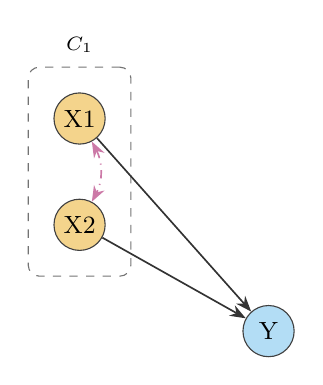
\begin{tikzpicture}
  \node[mannode] (nX1) at (0.00,0.00) {X1};
  \node[mannode] (nX2) at (0.00,-1.35) {X2};
  \node[tgtnode] (nY) at (2.40,-2.70) {Y};
  \draw[diredge] (nX1) -- (nY);
  \draw[diredge] (nX2) -- (nY);
  \draw[biintra] (nX1) to[bend left=28] (nX2);
  \begin{scope}[on background layer]
    \node[clbox,fit=(nX1)(nX2),label={[label distance=0.5mm]above:{\scriptsize$C_{1}$}}] {};
  \end{scope}
\end{tikzpicture}}\hfill
\adjustbox{max width=0.38\linewidth,valign=c}{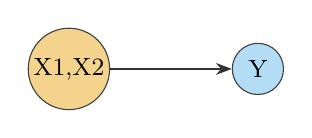
\begin{tikzpicture}
  \node[tgtnode] (nY) at (2.40,0.00) {Y};
  \node[mannode] (nX1X2) at (0.00,0.00) {X1,X2};
  \draw[diredge] (nX1X2) -- (nY);
\end{tikzpicture}}
\caption{\textbf{ParallelParent (MinimalBench, Exp.\ A).} Fine DAG with coarse partition (left) and quotient C-DAG (right), in the convention of Fig.~\ref{fig:motivating}: manipulable variables orange, target blue, dash-dotted latent confounding; dashed boxes are the manipulable clusters. The intra-cluster $X_1\leftrightarrow X_2$ disappears in the quotient; deleting $X_1\to Y$ leaves $C_1\to Y$ alive through $X_2\to Y$ (quotient-redundant).}
\label{fig:dag-parallelparent}
\end{figure}

\begin{figure}[t]\centering
\adjustbox{max width=0.58\linewidth,valign=c}{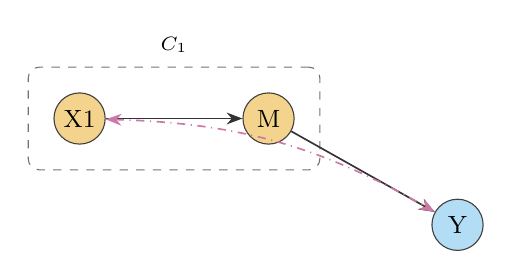
\begin{tikzpicture}
  \node[mannode] (nX1) at (0.00,0.00) {X1};
  \node[mannode] (nM) at (2.40,0.00) {M};
  \node[tgtnode] (nY) at (4.80,-1.35) {Y};
  \draw[diredge] (nX1) -- (nM);
  \draw[diredge] (nM) -- (nY);
  \draw[bicross] (nX1) to[bend left=14] (nY);
  \begin{scope}[on background layer]
    \node[clbox,fit=(nX1)(nM),label={[label distance=0.5mm]above:{\scriptsize$C_{1}$}}] {};
  \end{scope}
\end{tikzpicture}}\hfill
\adjustbox{max width=0.38\linewidth,valign=c}{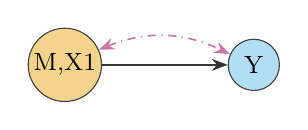
\begin{tikzpicture}
  \node[mannode] (nMX1) at (0.00,0.00) {M,X1};
  \node[tgtnode] (nY) at (2.40,0.00) {Y};
  \draw[diredge] (nMX1) -- (nY);
  \draw[bicross] (nMX1) to[bend left=24] (nY);
\end{tikzpicture}}
\caption{\textbf{FrontDoor (MinimalBench, Exp.\ B).} Fine DAG with coarse partition (left) and quotient C-DAG (right), in the convention of Fig.~\ref{fig:motivating}: manipulable variables orange, target blue, dash-dotted latent confounding; dashed boxes are the manipulable clusters. The quotient is a bow ($C_1\to Y$, $C_1\leftrightarrow Y$): the cluster arm runs on the uninformative prior tier in every condition, so the assumed intra-cluster $X_1\leftrightarrow M$ cannot change it.}
\label{fig:dag-frontdoor}
\end{figure}

\begin{figure}[t]\centering
\adjustbox{max width=0.58\linewidth,valign=c}{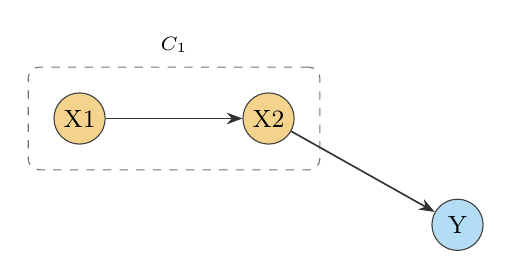
\begin{tikzpicture}
  \node[mannode] (nX1) at (0.00,0.00) {X1};
  \node[mannode] (nX2) at (2.40,0.00) {X2};
  \node[tgtnode] (nY) at (4.80,-1.35) {Y};
  \draw[diredge] (nX1) -- (nX2);
  \draw[diredge] (nX2) -- (nY);
  \begin{scope}[on background layer]
    \node[clbox,fit=(nX1)(nX2),label={[label distance=0.5mm]above:{\scriptsize$C_{1}$}}] {};
  \end{scope}
\end{tikzpicture}}\hfill
\adjustbox{max width=0.38\linewidth,valign=c}{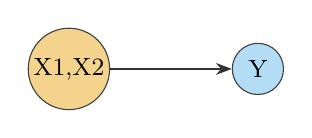
\begin{tikzpicture}
  \node[tgtnode] (nY) at (2.40,0.00) {Y};
  \node[mannode] (nX1X2) at (0.00,0.00) {X1,X2};
  \draw[diredge] (nX1X2) -- (nY);
\end{tikzpicture}}
\caption{\textbf{MediatedChain (MinimalBench, Exp.\ C).} Fine DAG with coarse partition (left) and quotient C-DAG (right), in the convention of Fig.~\ref{fig:motivating}: manipulable variables orange, target blue, dash-dotted latent confounding; dashed boxes are the manipulable clusters. The policy box restricts $D(X_2)$ to $[-2,2]$; the fine optimum $\doo(X_1{=}2)$ drives $X_2$ to $4$, outside the box.}
\label{fig:dag-mediatedchain}
\end{figure}

\begin{figure}[t]\centering
\adjustbox{max width=0.58\linewidth,valign=c}{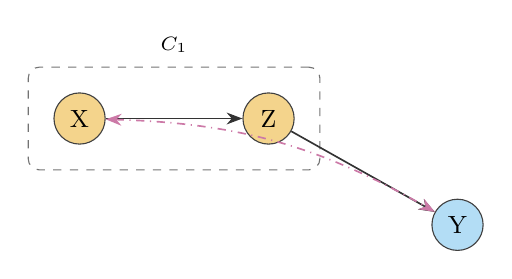
\begin{tikzpicture}
  \node[mannode] (nX) at (0.00,0.00) {X};
  \node[mannode] (nZ) at (2.40,0.00) {Z};
  \node[tgtnode] (nY) at (4.80,-1.35) {Y};
  \draw[diredge] (nX) -- (nZ);
  \draw[diredge] (nZ) -- (nY);
  \draw[bicross] (nX) to[bend left=14] (nY);
  \begin{scope}[on background layer]
    \node[clbox,fit=(nX)(nZ),label={[label distance=0.5mm]above:{\scriptsize$C_{1}$}}] {};
  \end{scope}
\end{tikzpicture}}\hfill
\adjustbox{max width=0.38\linewidth,valign=c}{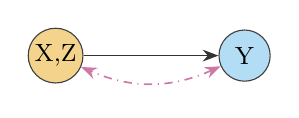
\begin{tikzpicture}
  \node[tgtnode] (nY) at (2.40,0.00) {Y};
  \node[mannode] (nXZ) at (0.00,0.00) {X,Z};
  \draw[diredge] (nXZ) -- (nY);
  \draw[bicross] (nY) to[bend left=24] (nXZ);
\end{tikzpicture}}
\caption{\textbf{ToyGraph (CBO family).} Fine DAG with coarse partition (left) and quotient C-DAG (right), in the convention of Fig.~\ref{fig:motivating}: manipulable variables orange, target blue, dash-dotted latent confounding; dashed boxes are the manipulable clusters. The quotient is a bow ($C_1\to Y$, $C_1\leftrightarrow Y$): $\doo(C_1)$ is not identifiable from the C-DAG, so the arm runs on the uninformative prior tier.}
\label{fig:dag-toy}
\end{figure}

\begin{figure}[t]\centering
\adjustbox{max width=0.58\linewidth,valign=c}{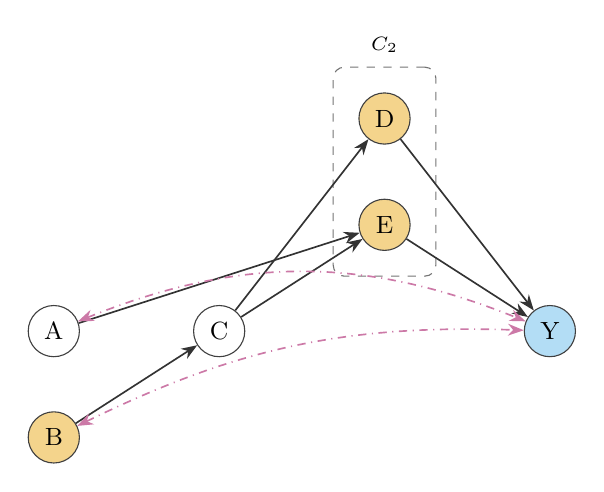
\begin{tikzpicture}
  \node[obsnode] (nA) at (0.00,-2.70) {A};
  \node[mannode] (nB) at (0.00,-4.05) {B};
  \node[obsnode] (nC) at (2.10,-2.70) {C};
  \node[mannode] (nD) at (4.20,0.00) {D};
  \node[mannode] (nE) at (4.20,-1.35) {E};
  \node[tgtnode] (nY) at (6.30,-2.70) {Y};
  \draw[diredge] (nB) -- (nC);
  \draw[diredge] (nC) -- (nD);
  \draw[diredge] (nA) -- (nE);
  \draw[diredge] (nC) -- (nE);
  \draw[diredge] (nD) -- (nY);
  \draw[diredge] (nE) -- (nY);
  \draw[bicross] (nB) to[bend left=14] (nY);
  \draw[bicross] (nA) to[bend left=22] (nY);
  \begin{scope}[on background layer]
    \node[clbox,fit=(nD)(nE),label={[label distance=0.5mm]above:{\scriptsize$C_{2}$}}] {};
  \end{scope}
\end{tikzpicture}}\hfill
\adjustbox{max width=0.38\linewidth,valign=c}{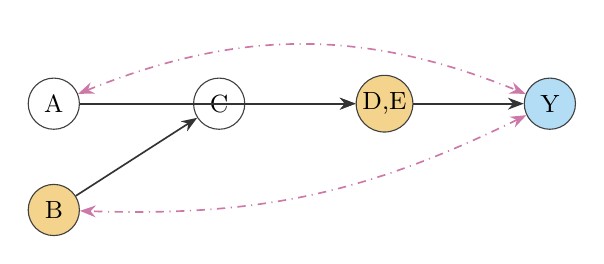
\begin{tikzpicture}
  \node[mannode] (nB) at (0.00,-1.35) {B};
  \node[obsnode] (nC) at (2.10,0.00) {C};
  \node[obsnode] (nA) at (0.00,0.00) {A};
  \node[mannode] (nDE) at (4.20,0.00) {D,E};
  \node[tgtnode] (nY) at (6.30,0.00) {Y};
  \draw[diredge] (nC) -- (nDE);
  \draw[diredge] (nB) -- (nC);
  \draw[diredge] (nA) -- (nDE);
  \draw[diredge] (nDE) -- (nY);
  \draw[bicross] (nY) to[bend left=14] (nB);
  \draw[bicross] (nA) to[bend left=22] (nY);
\end{tikzpicture}}
\caption{\textbf{CompleteGraph (CBO family).} Fine DAG with coarse partition (left) and quotient C-DAG (right), in the convention of Fig.~\ref{fig:motivating}: manipulable variables orange, target blue, dash-dotted latent confounding; dashed boxes are the manipulable clusters.}
\label{fig:dag-complete}
\end{figure}

\begin{figure}[t]\centering
\adjustbox{max width=0.58\linewidth,valign=c}{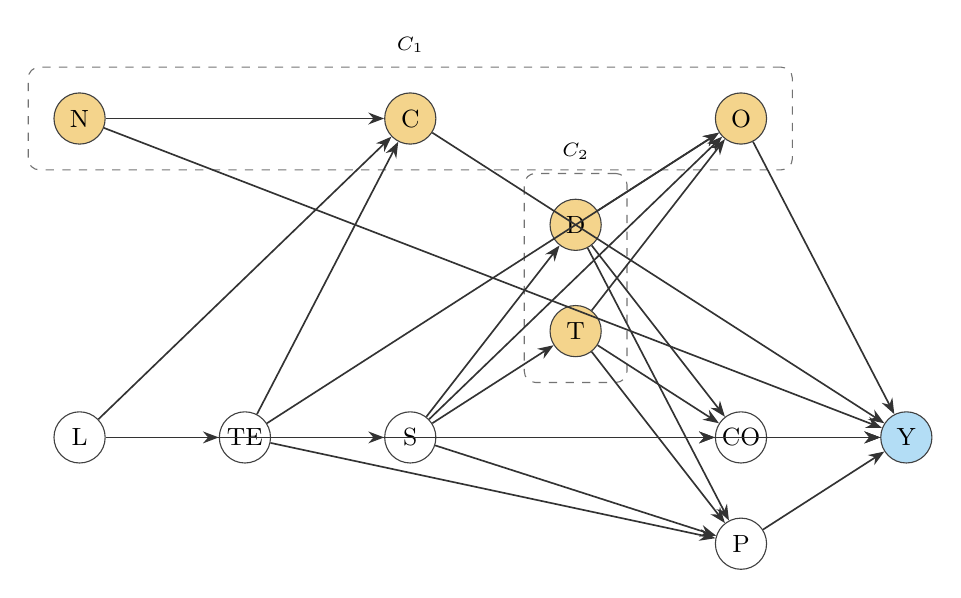
\begin{tikzpicture}
  \node[mannode] (nN) at (0.00,0.00) {N};
  \node[obsnode] (nL) at (0.00,-4.05) {L};
  \node[obsnode] (nTE) at (2.10,-4.05) {TE};
  \node[mannode] (nC) at (4.20,0.00) {C};
  \node[obsnode] (nS) at (4.20,-4.05) {S};
  \node[mannode] (nT) at (6.30,-2.70) {T};
  \node[mannode] (nD) at (6.30,-1.35) {D};
  \node[obsnode] (nP) at (8.40,-5.40) {P};
  \node[mannode] (nO) at (8.40,0.00) {O};
  \node[obsnode] (nCO) at (8.40,-4.05) {CO};
  \node[tgtnode] (nY) at (10.50,-4.05) {Y};
  \draw[diredge] (nL) -- (nTE);
  \draw[diredge] (nL) -- (nC);
  \draw[diredge] (nL) -- (nY);
  \draw[diredge] (nN) -- (nC);
  \draw[diredge] (nN) -- (nY);
  \draw[diredge] (nTE) -- (nC);
  \draw[diredge] (nTE) -- (nS);
  \draw[diredge] (nTE) -- (nP);
  \draw[diredge] (nTE) -- (nO);
  \draw[diredge] (nTE) -- (nCO);
  \draw[diredge] (nTE) -- (nY);
  \draw[diredge] (nS) -- (nT);
  \draw[diredge] (nS) -- (nD);
  \draw[diredge] (nS) -- (nP);
  \draw[diredge] (nS) -- (nO);
  \draw[diredge] (nS) -- (nCO);
  \draw[diredge] (nT) -- (nP);
  \draw[diredge] (nT) -- (nO);
  \draw[diredge] (nT) -- (nCO);
  \draw[diredge] (nD) -- (nP);
  \draw[diredge] (nD) -- (nO);
  \draw[diredge] (nD) -- (nCO);
  \draw[diredge] (nP) -- (nY);
  \draw[diredge] (nO) -- (nY);
  \draw[diredge] (nC) -- (nY);
  \draw[diredge] (nCO) -- (nY);
  \begin{scope}[on background layer]
    \node[clbox,fit=(nC)(nN)(nO),label={[label distance=0.5mm]above:{\scriptsize$C_{1}$}}] {};
  \end{scope}
  \begin{scope}[on background layer]
    \node[clbox,fit=(nD)(nT),label={[label distance=0.5mm]above:{\scriptsize$C_{2}$}}] {};
  \end{scope}
\end{tikzpicture}}\hfill
\adjustbox{max width=0.38\linewidth,valign=c}{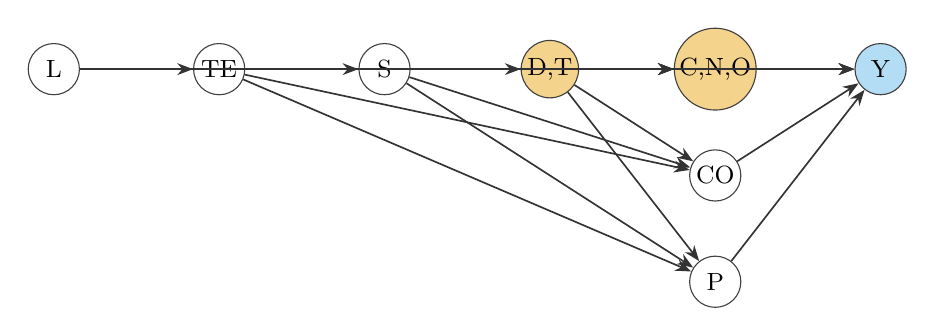
\begin{tikzpicture}
  \node[mannode] (nDT) at (6.30,0.00) {D,T};
  \node[obsnode] (nTE) at (2.10,0.00) {TE};
  \node[mannode] (nCNO) at (8.40,0.00) {C,N,O};
  \node[obsnode] (nS) at (4.20,0.00) {S};
  \node[obsnode] (nCO) at (8.40,-1.35) {CO};
  \node[obsnode] (nP) at (8.40,-2.70) {P};
  \node[obsnode] (nL) at (0.00,0.00) {L};
  \node[tgtnode] (nY) at (10.50,0.00) {Y};
  \draw[diredge] (nL) -- (nY);
  \draw[diredge] (nS) -- (nCNO);
  \draw[diredge] (nCNO) -- (nY);
  \draw[diredge] (nTE) -- (nCNO);
  \draw[diredge] (nTE) -- (nP);
  \draw[diredge] (nDT) -- (nCNO);
  \draw[diredge] (nS) -- (nCO);
  \draw[diredge] (nL) -- (nTE);
  \draw[diredge] (nP) -- (nY);
  \draw[diredge] (nDT) -- (nCO);
  \draw[diredge] (nTE) -- (nCO);
  \draw[diredge] (nDT) -- (nP);
  \draw[diredge] (nL) -- (nCNO);
  \draw[diredge] (nS) -- (nP);
  \draw[diredge] (nCO) -- (nY);
  \draw[diredge] (nS) -- (nDT);
  \draw[diredge] (nTE) -- (nY);
  \draw[diredge] (nTE) -- (nS);
\end{tikzpicture}}
\caption{\textbf{SimplifiedCoralGraph (CBO family).} Fine DAG with coarse partition (left) and quotient C-DAG (right), in the convention of Fig.~\ref{fig:motivating}: manipulable variables orange, target blue, dash-dotted latent confounding; dashed boxes are the manipulable clusters.}
\label{fig:dag-coral}
\end{figure}

\begin{figure}[t]\centering
\adjustbox{max width=0.58\linewidth,valign=c}{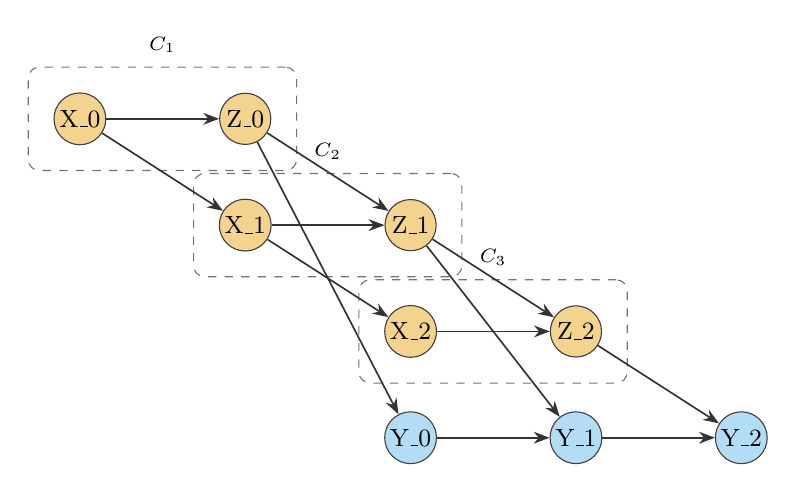
\begin{tikzpicture}
  \node[mannode] (nX0) at (0.00,0.00) {X\_0};
  \node[mannode] (nZ0) at (2.10,0.00) {Z\_0};
  \node[tgtnode] (nY0) at (4.20,-4.05) {Y\_0};
  \node[mannode] (nX1) at (2.10,-1.35) {X\_1};
  \node[mannode] (nZ1) at (4.20,-1.35) {Z\_1};
  \node[tgtnode] (nY1) at (6.30,-4.05) {Y\_1};
  \node[mannode] (nX2) at (4.20,-2.70) {X\_2};
  \node[mannode] (nZ2) at (6.30,-2.70) {Z\_2};
  \node[tgtnode] (nY2) at (8.40,-4.05) {Y\_2};
  \draw[diredge] (nX0) -- (nZ0);
  \draw[diredge] (nZ0) -- (nY0);
  \draw[diredge] (nX1) -- (nZ1);
  \draw[diredge] (nZ1) -- (nY1);
  \draw[diredge] (nX2) -- (nZ2);
  \draw[diredge] (nZ2) -- (nY2);
  \draw[diredge] (nX0) -- (nX1);
  \draw[diredge] (nZ0) -- (nZ1);
  \draw[diredge] (nY0) -- (nY1);
  \draw[diredge] (nX1) -- (nX2);
  \draw[diredge] (nZ1) -- (nZ2);
  \draw[diredge] (nY1) -- (nY2);
  \begin{scope}[on background layer]
    \node[clbox,fit=(nX0)(nZ0),label={[label distance=0.5mm]above:{\scriptsize$C_{1}$}}] {};
  \end{scope}
  \begin{scope}[on background layer]
    \node[clbox,fit=(nX1)(nZ1),label={[label distance=0.5mm]above:{\scriptsize$C_{2}$}}] {};
  \end{scope}
  \begin{scope}[on background layer]
    \node[clbox,fit=(nX2)(nZ2),label={[label distance=0.5mm]above:{\scriptsize$C_{3}$}}] {};
  \end{scope}
\end{tikzpicture}}\hfill
\adjustbox{max width=0.38\linewidth,valign=c}{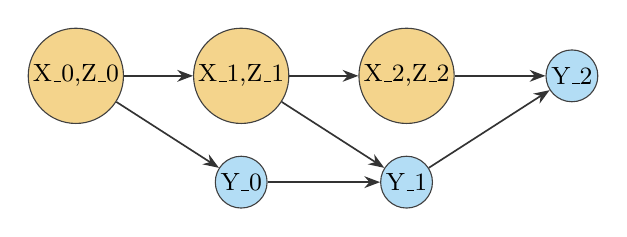
\begin{tikzpicture}
  \node[mannode] (nX0Z0) at (0.00,0.00) {X\_0,Z\_0};
  \node[tgtnode] (nY0) at (2.10,-1.35) {Y\_0};
  \node[mannode] (nX1Z1) at (2.10,0.00) {X\_1,Z\_1};
  \node[tgtnode] (nY1) at (4.20,-1.35) {Y\_1};
  \node[mannode] (nX2Z2) at (4.20,0.00) {X\_2,Z\_2};
  \node[tgtnode] (nY2) at (6.30,0.00) {Y\_2};
  \draw[diredge] (nX0Z0) -- (nY0);
  \draw[diredge] (nX1Z1) -- (nY1);
  \draw[diredge] (nX2Z2) -- (nY2);
  \draw[diredge] (nX0Z0) -- (nX1Z1);
  \draw[diredge] (nY0) -- (nY1);
  \draw[diredge] (nX1Z1) -- (nX2Z2);
  \draw[diredge] (nY1) -- (nY2);
\end{tikzpicture}}
\caption{\textbf{DCBO stat / nonstat (QDCBO family).} Fine DAG with coarse partition (left) and quotient C-DAG (right), in the convention of Fig.~\ref{fig:motivating}: manipulable variables orange, target blue, dash-dotted latent confounding; dashed boxes are the manipulable clusters. Slices $t=0,1,2$; the nonstat setup shares this topology with a change point in the SEM.}
\label{fig:dag-dcbo-stat}
\end{figure}

\begin{figure}[t]\centering
\adjustbox{max width=0.58\linewidth,valign=c}{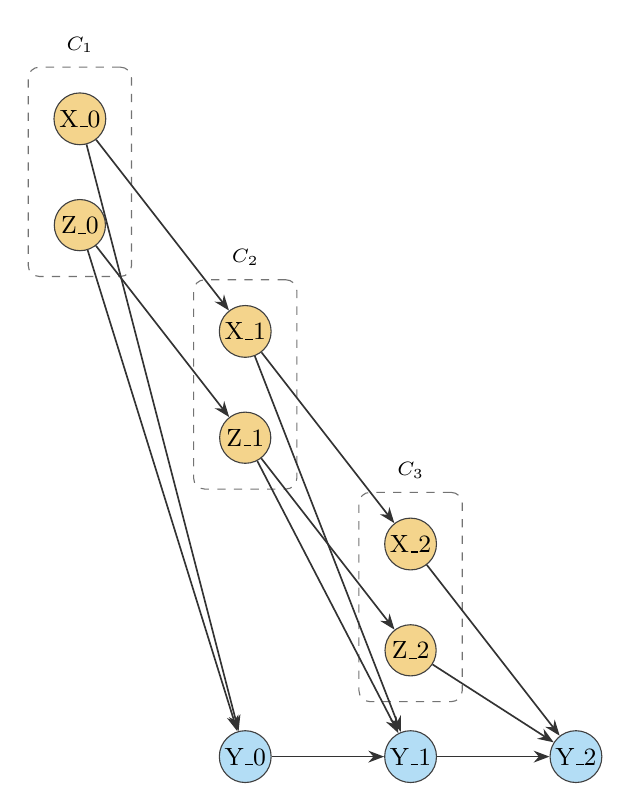
\begin{tikzpicture}
  \node[mannode] (nX0) at (0.00,0.00) {X\_0};
  \node[mannode] (nZ0) at (0.00,-1.35) {Z\_0};
  \node[tgtnode] (nY0) at (2.10,-8.10) {Y\_0};
  \node[mannode] (nX1) at (2.10,-2.70) {X\_1};
  \node[mannode] (nZ1) at (2.10,-4.05) {Z\_1};
  \node[tgtnode] (nY1) at (4.20,-8.10) {Y\_1};
  \node[mannode] (nX2) at (4.20,-5.40) {X\_2};
  \node[mannode] (nZ2) at (4.20,-6.75) {Z\_2};
  \node[tgtnode] (nY2) at (6.30,-8.10) {Y\_2};
  \draw[diredge] (nX0) -- (nY0);
  \draw[diredge] (nZ0) -- (nY0);
  \draw[diredge] (nX1) -- (nY1);
  \draw[diredge] (nZ1) -- (nY1);
  \draw[diredge] (nX2) -- (nY2);
  \draw[diredge] (nZ2) -- (nY2);
  \draw[diredge] (nX0) -- (nX1);
  \draw[diredge] (nZ0) -- (nZ1);
  \draw[diredge] (nY0) -- (nY1);
  \draw[diredge] (nX1) -- (nX2);
  \draw[diredge] (nZ1) -- (nZ2);
  \draw[diredge] (nY1) -- (nY2);
  \begin{scope}[on background layer]
    \node[clbox,fit=(nX0)(nZ0),label={[label distance=0.5mm]above:{\scriptsize$C_{1}$}}] {};
  \end{scope}
  \begin{scope}[on background layer]
    \node[clbox,fit=(nX1)(nZ1),label={[label distance=0.5mm]above:{\scriptsize$C_{2}$}}] {};
  \end{scope}
  \begin{scope}[on background layer]
    \node[clbox,fit=(nX2)(nZ2),label={[label distance=0.5mm]above:{\scriptsize$C_{3}$}}] {};
  \end{scope}
\end{tikzpicture}}\hfill
\adjustbox{max width=0.38\linewidth,valign=c}{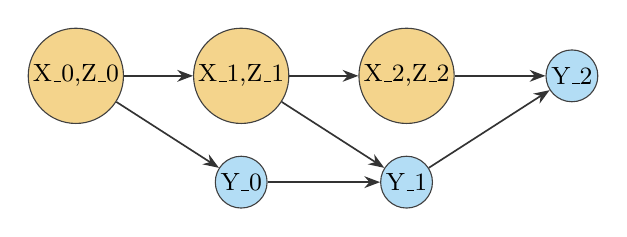
\begin{tikzpicture}
  \node[mannode] (nX0Z0) at (0.00,0.00) {X\_0,Z\_0};
  \node[tgtnode] (nY0) at (2.10,-1.35) {Y\_0};
  \node[mannode] (nX1Z1) at (2.10,0.00) {X\_1,Z\_1};
  \node[tgtnode] (nY1) at (4.20,-1.35) {Y\_1};
  \node[mannode] (nX2Z2) at (4.20,0.00) {X\_2,Z\_2};
  \node[tgtnode] (nY2) at (6.30,0.00) {Y\_2};
  \draw[diredge] (nX0Z0) -- (nY0);
  \draw[diredge] (nX1Z1) -- (nY1);
  \draw[diredge] (nX2Z2) -- (nY2);
  \draw[diredge] (nX0Z0) -- (nX1Z1);
  \draw[diredge] (nY0) -- (nY1);
  \draw[diredge] (nX1Z1) -- (nX2Z2);
  \draw[diredge] (nY1) -- (nY2);
\end{tikzpicture}}
\caption{\textbf{DCBO ind (QDCBO family).} Fine DAG with coarse partition (left) and quotient C-DAG (right), in the convention of Fig.~\ref{fig:motivating}: manipulable variables orange, target blue, dash-dotted latent confounding; dashed boxes are the manipulable clusters.}
\label{fig:dag-dcbo-ind}
\end{figure}

\begin{figure}[t]\centering
\adjustbox{max width=0.58\linewidth,valign=c}{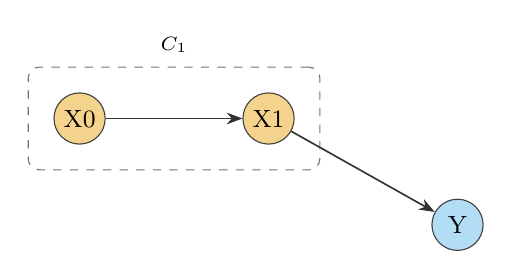
\begin{tikzpicture}
  \node[mannode] (nX0) at (0.00,0.00) {X0};
  \node[mannode] (nX1) at (2.40,0.00) {X1};
  \node[tgtnode] (nY) at (4.80,-1.35) {Y};
  \draw[diredge] (nX0) -- (nX1);
  \draw[diredge] (nX1) -- (nY);
  \begin{scope}[on background layer]
    \node[clbox,fit=(nX0)(nX1),label={[label distance=0.5mm]above:{\scriptsize$C_{1}$}}] {};
  \end{scope}
\end{tikzpicture}}\hfill
\adjustbox{max width=0.38\linewidth,valign=c}{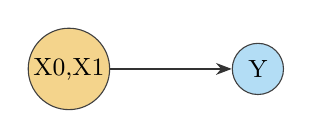
\begin{tikzpicture}
  \node[mannode] (nX0X1) at (0.00,0.00) {X0,X1};
  \node[tgtnode] (nY) at (2.40,0.00) {Y};
  \draw[diredge] (nX0X1) -- (nY);
\end{tikzpicture}}
\caption{\textbf{ToyGraph-M (QMCBO family).} Fine DAG with coarse partition (left) and quotient C-DAG (right), in the convention of Fig.~\ref{fig:motivating}: manipulable variables orange, target blue, dash-dotted latent confounding; dashed boxes are the manipulable clusters.}
\label{fig:dag-mcbo-toygraph-m}
\end{figure}

\begin{figure}[t]\centering
\adjustbox{max width=0.58\linewidth,valign=c}{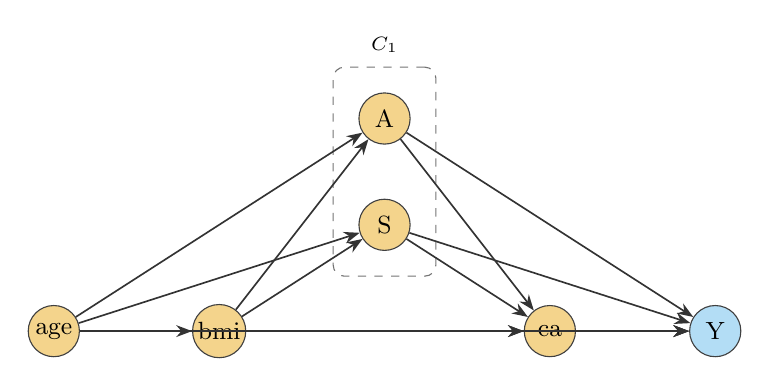
\begin{tikzpicture}
  \node[mannode] (nage) at (0.00,-2.70) {age};
  \node[mannode] (nbmi) at (2.10,-2.70) {bmi};
  \node[mannode] (nA) at (4.20,0.00) {A};
  \node[mannode] (nS) at (4.20,-1.35) {S};
  \node[mannode] (nca) at (6.30,-2.70) {ca};
  \node[tgtnode] (nY) at (8.40,-2.70) {Y};
  \draw[diredge] (nage) -- (nbmi);
  \draw[diredge] (nage) -- (nA);
  \draw[diredge] (nbmi) -- (nA);
  \draw[diredge] (nage) -- (nS);
  \draw[diredge] (nbmi) -- (nS);
  \draw[diredge] (nage) -- (nca);
  \draw[diredge] (nbmi) -- (nca);
  \draw[diredge] (nA) -- (nca);
  \draw[diredge] (nS) -- (nca);
  \draw[diredge] (nage) -- (nY);
  \draw[diredge] (nbmi) -- (nY);
  \draw[diredge] (nA) -- (nY);
  \draw[diredge] (nS) -- (nY);
  \draw[diredge] (nca) -- (nY);
  \begin{scope}[on background layer]
    \node[clbox,fit=(nA)(nS),label={[label distance=0.5mm]above:{\scriptsize$C_{1}$}}] {};
  \end{scope}
\end{tikzpicture}}\hfill
\adjustbox{max width=0.38\linewidth,valign=c}{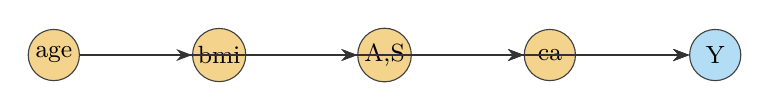
\begin{tikzpicture}
  \node[mannode] (nage) at (0.00,0.00) {age};
  \node[mannode] (nbmi) at (2.10,0.00) {bmi};
  \node[mannode] (nAS) at (4.20,0.00) {A,S};
  \node[mannode] (nca) at (6.30,0.00) {ca};
  \node[tgtnode] (nY) at (8.40,0.00) {Y};
  \draw[diredge] (nage) -- (nbmi);
  \draw[diredge] (nage) -- (nAS);
  \draw[diredge] (nbmi) -- (nAS);
  \draw[diredge] (nage) -- (nca);
  \draw[diredge] (nbmi) -- (nca);
  \draw[diredge] (nAS) -- (nca);
  \draw[diredge] (nage) -- (nY);
  \draw[diredge] (nbmi) -- (nY);
  \draw[diredge] (nAS) -- (nY);
  \draw[diredge] (nca) -- (nY);
\end{tikzpicture}}
\caption{\textbf{PSAGraph (QMCBO family).} Fine DAG with coarse partition (left) and quotient C-DAG (right), in the convention of Fig.~\ref{fig:motivating}: manipulable variables orange, target blue, dash-dotted latent confounding; dashed boxes are the manipulable clusters.}
\label{fig:dag-mcbo-psagraph}
\end{figure}



\section{Implementation and reproducibility}\label{app:repro}

\begin{algorithm}[t]
\caption{\QCBO{}: Quotient Causal Bayesian Optimization}
\label{alg:ccbo}
\begin{algorithmic}[1]
\REQUIRE C-DAG $\Gq$ over the clusters of $\Pi$ (or a fine hypothesis $\Gg$ and
$\Pi$); target $Y$; number of trials $T$; observational pool
$\mathcal{D}^{O}_{\mathrm{full}}$ with initial slice $\mathcal{D}^{O}_0$, batch size
$b$ and budget $N_{\mathrm{cap}}$; optional hierarchy $\mathcal H$
(\S\ref{sec:refine}).
\STATE If given $\Gg$: $\Gg^*\leftarrow$ latent projection of $\Gg$;\quad
$\Gq\leftarrow$ quotient of $\Gg^*$ under $\Pi$. Check acyclicity of $\Gq$
(Assumption~\ref{ass:valid}).
\STATE Build $\ESpi \leftarrow \mathrm{MIS}(\Gq)$ via
Eq.~\eqref{eq:ccbo_exploration}.
\STATE For each $\mathbf{X}_s\in\ESpi$: run complete ID on
$P(Y\mid\doo(\mathbf{X}_s))$ and fit the prior mean $m_s$ via the two-tier
rule, Eq.~\eqref{eq:two_tier_prior}, on $\mathcal{D}^{O}$.
\STATE Collect initial interventional data $\mathcal{D}^{I}_0$.
\FOR{$t=1,\ldots,T$}
  \STATE $c\leftarrow(N_t<N_{\mathrm{cap}})$ \COMMENT{observational budget left}
  \IF{$c$ \AND ($t$ is the first trial of a phase \OR $u\sim U[0,1)<\epsilon_t$,
  Eq.~\eqref{eq:eps})}
    \STATE Reveal the next unseen batch $\mathcal{D}^{O}_{t}\leftarrow
    \mathcal{D}^{O}_{t-1}\cup\{\text{next }b\text{ rows, truncated at }N_{\mathrm{cap}}\}$.
    \STATE Re-fit the identified functionals on $\mathcal{D}^{O}_{t}$ and rebuild
    every prior mean $m_s$, Eq.~\eqref{eq:two_tier_prior}. \textbf{continue}
  \ENDIF
  \STATE Update GP posteriors $(m_{s,t},k_{s,t})$ for all $\mathbf{X}_s\in\ESpi$.
  \STATE $(\mathbf{X}_{s_t},\mathbf{x}_t)\leftarrow\arg\max_{s,\mathbf{x}}
  \mathrm{EI}^{s}_{t}(\mathbf{x})/Co(\mathbf{X}_s,\mathbf{x})$.
  \STATE Intervene, observe $y_t$; update $\mathcal{D}^{I}_t$.
  \STATE \textbf{if} $\mathcal H$ declared \textbf{and} incumbent plateaued: split the
  incumbent's clusters via $\mathcal H$, re-check validity, rebuild
  $\ESpi\,\cup$ past arms, carry $\mathcal{D}^{I}_t$ and $(\mathcal{D}^{O}_t,
  \text{pool cursor})$ (\S\ref{sec:refine}), init new arms.
\ENDFOR
\RETURN $(\mathbf{X}_{s_{t^\star}},\mathbf{x}_{t^\star})$ where $t^\star=\arg\min_t y_t$.
\end{algorithmic}
\end{algorithm}

All methods share one surrogate/acquisition backend (the vendored \CBO{} loop), so
comparisons differ only in the assumed structure. \textbf{Surrogate.} Each
exploration-set arm carries a \textsc{GPy} \texttt{GPRegression} model with an RBF
kernel (signal variance and lengthscale initialized to $1$, ARD off) and observation
noise fixed near zero ($10^{-10}$, matching the deterministic mechanisms). The causal
prior supplies the do-calculus estimate as the GP \emph{mean function}, so
$\Delta$-metrics isolate the effect of a wrong prior/exploration set from surrogate
noise. \textbf{Acquisition.} Causal expected improvement \citep{garnettBayesianOptimization2023}, maximized
over the box-constrained intervention domain by gradient-based L-BFGS.
\textbf{Protocol (minimal suite).} Unit per-variable intervention costs,
$3$ initial interventional points per arm, $T{=}50$ trials ($60$ on
\textsc{MediatedChain}), $30$ seeds, $n_{\mathrm{obs}}{=}100$ from one
shared dataset per SCM; the family suite follows each base paper's own
protocol (\S\ref{sec:exp-d}). Every run additionally logs the selected arm
and intervention values per trial, so invariance is checked on
\emph{decisions}, not only on incumbent values.

\textbf{Observation protocol.} A trial is either an \emph{observation} or an
\emph{intervention}. The run starts from $n_{\mathrm{obs}}{=}100$
observational rows; each observation action reveals a fresh batch of $20$
previously unseen rows from the same shared pool, the final batch being
truncated at the budget $N_{\max}{=}150$ (so at most $50$ rows are acquired
online). Once $N_t{=}N_{\mathrm{cap}}{=}\min(N_{\max},|\mathcal D^{O}_{\mathrm{full}}|)$
the optimizer must intervene. Every observation refreshes the identified
functionals of Eq.~\eqref{eq:two_tier_prior} on the enlarged dataset and
rebuilds each arm's GP prior. We follow the released \CBO{} implementation's
observe/intervene schedule: at trial $t$ it observes with probability
\begin{equation}
\epsilon_t=\operatorname{clip}_{[0,1]}\!\left[
\frac{\operatorname{Vol}(\mathcal C(\mathcal D^{O}_t))}{\operatorname{Vol}(\mathcal D(\mathbf X))}
\bigg/ \frac{N_t}{N_{\mathrm{cap}}}\right],
\label{eq:eps}
\end{equation}
subject to the remaining budget, and the first trial of a phase observes if
budget remains.\footnote{The division in Eq.~\eqref{eq:eps} follows the
reference implementation and differs from the multiplication-based expression
printed in \citet{agliettiCausalBayesianOptimization2020b}. The difference is measurable rather
than cosmetic --- on \textsc{ParallelParent} at $N_t{=}100$ the two give
$\epsilon_t\approx0.11$ and $0.05$ --- so we state which one we ran. Because
every causal arm shares this backend, the schedule is common to \CBO{},
\QCBO{} and \HQCBO{} alike; \BO{} takes no observation actions at all.}

\textbf{\BO{} baseline.} Standard Bayesian optimization over a single joint
arm on all manipulable variables, with no causal prior and no observation
actions. It reads no graph structure, so its trajectory is \emph{identical}
across every misspecification condition of an SCM: it is the
``invariance for free, no causal prior'' corner of
Table~\ref{tab:minimal-taxonomy}, and the reference for what the causal prior
buys rather than a competitor for the invariance claim. Note it intervenes on
every manipulable variable each trial, so under unit per-variable costs it
pays $|\mathbf X|$ per trial against a causal method's per-arm cost; the
cost-indexed panels must be read with that in mind.
\textbf{Invariance tolerance.} Arm-choice and intervention-value sequences
are compared exactly; incumbent trajectories at $10^{-8}$ (GP-solver
floating point). On every protected condition of
Table~\ref{tab:minimal-taxonomy} the sequences are identical and
$\sup|\Delta|=0$; the quotient-visible control moves trajectories on every
seed.
\textbf{Artifacts.} The MinimalBench structural module
(\texttt{ccbo/minibench.py}), its data generators with built-in oracle
gates, the dataset-free structural tests and end-to-end invariance
regressions, the suite runner (\texttt{scripts/run\_minimal\_suite.py}),
the native two-phase \HQCBO{} (\texttt{ccbo/minimal\_suite.py}), and every
table/figure emitter are released, so all reported numbers regenerate from
the released SCMs and seeds.

\paragraph{Initialization-inclusive cost accounting.}
Reported cumulative costs exclude the initial design (three
interventional points per arm on MinimalBench, ten on the \CBO{}
family; per-variable unit costs), so methods with different arm counts
consume different unlogged budgets at equal $T$. Table~\ref{tab:cost}
reconstructs, per method, the exploration-set size, initialization
cost, logged cost, and total, and re-evaluates each method at the
matched budget $C^\ast$, the smallest total across the group's methods.
\HQCBO{} additionally pays three points per arm exposed at
its per-seed split. The trajectory \emph{through} initialization is
unlogged and is not reconstructed: each curve starts at its
post-initialization incumbent placed at its full initialization cost,
and budgets below that are reported as unavailable. Two reversals are
worth naming: on Synthetic, \CBO{}'s final-value advantage over
\QCBO{} disappears at matched total cost, and on Coral, \CBO{}'s
$31$-arm initialization ($800$ cost units) exceeds \QCBO{}'s entire
total budget. On \textsc{FrontDoor} the comparison moves the other
way: fine \CBO{} reaches the well within a smaller total budget. The
DCBO and MCBO families follow their base papers' trial-indexed
protocols and are not re-costed.

\begin{table}[t]\centering
  \caption{Initialization-inclusive cost accounting and matched-budget
  comparison (means over seeds; $Y$ at $C^\ast$ by step interpolation
  above the post-initialization incumbent; ``n/a'' = initialization
  alone exceeds $C^\ast$).}
  \label{tab:cost}
  \small
  \adjustbox{max width=\linewidth}{% Auto-generated by scripts/emit_cost_analysis.py -- do not edit.
\begin{tabular}{@{}lcccccc@{}}
\toprule
\textbf{Method} & $|\mathrm{ES}|$ & \textbf{Init} & \textbf{Logged} & \textbf{Total} & \textbf{Final $Y$} & \textbf{$Y$ at $C^\ast$} \\
\midrule
\multicolumn{7}{@{}l}{\emph{ParallelParent A0 (correct) ($C^\ast{=}73$)}} \\
CBO & 3 & 12 & 86 & 98 & $0.001{\scriptstyle\,\pm\,}0.000$ & $0.003{\scriptstyle\,\pm\,}0.001$ \\
QCBO & 1 & 6 & 94 & 100 & $0.002{\scriptstyle\,\pm\,}0.000$ & $0.003{\scriptstyle\,\pm\,}0.001$ \\
CEO & 3 & 12 & 61 & 73 & $1.001{\scriptstyle\,\pm\,}0.304$ & $1.011{\scriptstyle\,\pm\,}0.303$ \\
\addlinespace[2pt]
\multicolumn{7}{@{}l}{\emph{ParallelParent A1 (del $X_1{\to}Y$) ($C^\ast{=}50$)}} \\
CBO & 1 & 3 & 47 & 50 & $4.250{\scriptstyle\,\pm\,}0.000$ & $4.250{\scriptstyle\,\pm\,}0.000$ \\
QCBO & 1 & 6 & 94 & 100 & $0.002{\scriptstyle\,\pm\,}0.000$ & $0.004{\scriptstyle\,\pm\,}0.001$ \\
CEO & 3 & 12 & 62 & 74 & $0.773{\scriptstyle\,\pm\,}0.258$ & $0.792{\scriptstyle\,\pm\,}0.256$ \\
\addlinespace[2pt]
\multicolumn{7}{@{}l}{\emph{FrontDoor B0 (correct) ($C^\ast{=}53$)}} \\
CBO & 2 & 6 & 47 & 53 & $0.000{\scriptstyle\,\pm\,}0.000$ & $0.000{\scriptstyle\,\pm\,}0.000$ \\
QCBO & 1 & 6 & 94 & 100 & $0.001{\scriptstyle\,\pm\,}0.001$ & $0.013{\scriptstyle\,\pm\,}0.005$ \\
CEO & 3 & 12 & 58 & 70 & $0.070{\scriptstyle\,\pm\,}0.023$ & $0.097{\scriptstyle\,\pm\,}0.030$ \\
\addlinespace[2pt]
\multicolumn{7}{@{}l}{\emph{MediatedChain C0 ($C^\ast{=}63$)}} \\
CBO & 2 & 6 & 57 & 63 & $0.040{\scriptstyle\,\pm\,}0.000$ & $0.040{\scriptstyle\,\pm\,}0.000$ \\
QCBO & 1 & 6 & 114 & 120 & $4.000{\scriptstyle\,\pm\,}0.000$ & $4.000{\scriptstyle\,\pm\,}0.000$ \\
HQCBO & 1 & 6$+$6 & 79 & 91 & $0.040{\scriptstyle\,\pm\,}0.000$ & $0.040{\scriptstyle\,\pm\,}0.000$ \\
CEO & 3 & 12 & 114 & 126 & $0.135{\scriptstyle\,\pm\,}0.035$ & $0.212{\scriptstyle\,\pm\,}0.060$ \\
\addlinespace[2pt]
\multicolumn{7}{@{}l}{\emph{Toy (family suite) ($C^\ast{=}57$)}} \\
CBO & 2 & 20 & 37 & 57 & $-2.164{\scriptstyle\,\pm\,}0.000$ & $-2.164{\scriptstyle\,\pm\,}0.000$ \\
QCBO & 1 & 20 & 74 & 94 & $-2.169{\scriptstyle\,\pm\,}0.005$ & $-2.072{\scriptstyle\,\pm\,}0.049$ \\
\addlinespace[2pt]
\multicolumn{7}{@{}l}{\emph{Synthetic (family suite) ($C^\ast{=}99$)}} \\
CBO & 6 & 90 & 67 & 157 & $-3.472{\scriptstyle\,\pm\,}0.041$ & $-1.801{\scriptstyle\,\pm\,}0.290$ \\
QCBO & 2 & 30 & 69 & 99 & $-1.285{\scriptstyle\,\pm\,}0.029$ & $-1.285{\scriptstyle\,\pm\,}0.029$ \\
\addlinespace[2pt]
\multicolumn{7}{@{}l}{\emph{Coral (family suite) ($C^\ast{=}217$)}} \\
CBO & 31 & 800 & 96 & 896 & $36.065{\scriptstyle\,\pm\,}0.018$ & n/a \\
QCBO & 3 & 100 & 117 & 217 & $36.449{\scriptstyle\,\pm\,}0.017$ & $36.449{\scriptstyle\,\pm\,}0.017$ \\
\bottomrule
\end{tabular}
}
\end{table}

\paragraph{Reproducibility statement.}
The repository archives the complete raw per-seed traces behind every
figure and table (\texttt{artifacts/traces/}: five compressed archives
with per-file SHA256 checksums and a provenance manifest recording
source commits, generating scripts, and settings), pip-freeze
snapshots of both experiment environments with platform details and
pinned external-stack commits (\texttt{envs/}), and a verification
gate (\texttt{scripts/verify\_traces.py}) that re-checks the archive's
file grid, recomputes every reported aggregate at displayed precision,
and re-tests the exact invariance predictions. One command
(\texttt{scripts/reproduce\_paper.sh}) regenerates every figure and
table from the archives into a fresh working directory and rebuilds
this document.

\section{Full results}\label{app:fulltables}
Figure~\ref{fig:family} and Table~\ref{tab:family} give the full family-suite
curves and paired effects behind \S\ref{sec:exp-d}. Tables~\ref{tab:qmcbo-e1}
and~\ref{tab:qmcbo-e2} give the model-based detail: finals, wall-clock, and
invariance under an intra-cluster perturbation of the model's graph view.
Per-seed CSVs for every minimal-suite unit (trial,
incumbent, cumulative cost, selected arm, and intervention values)
regenerate from the archived traces (App.~\ref{app:repro}).

\begin{figure*}[t]\centering
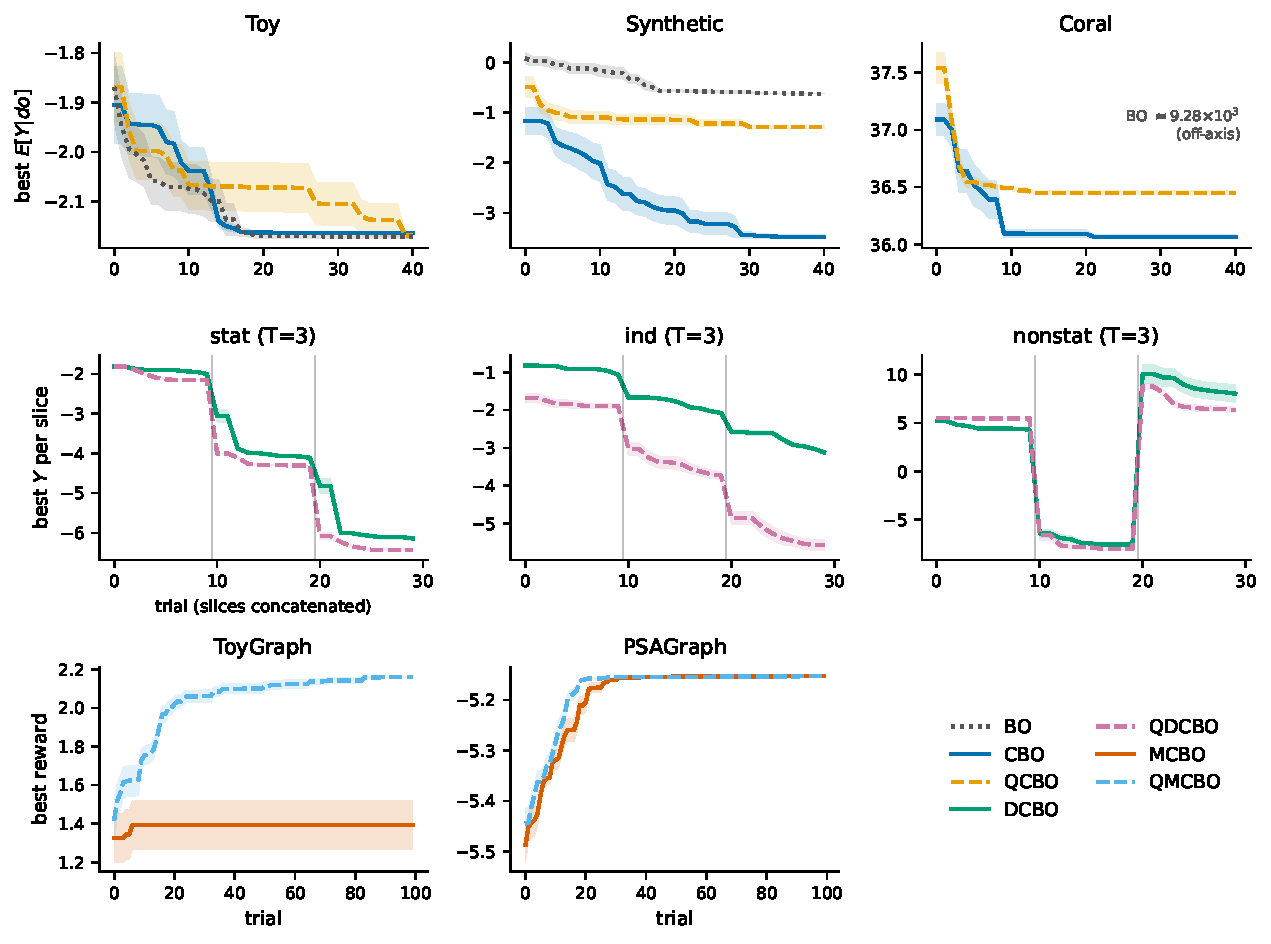
\includegraphics[width=\textwidth]{figures/family_suite}
\caption{Quotient methods and their bases on the base papers' benchmarks,
mean$\pm$s.e. Top: minimization for \CBO{}. Middle: DCBO slices. Bottom:
maximization for MCBO.}
\label{fig:family}
\end{figure*}

\begin{table*}[t]\centering
  \caption{Family suite: finals and per-task \emph{paired}
  final-performance effects $\Delta$ (quotient $-$ base in the task's
  own direction; positive = quotient worse) with paired-$t$ $95\%$
  CIs. These are finite-budget empirical effects, not estimates of the
  action-space gap $\Delta(\Pi)$.}
  \label{tab:family}
  \small
  % Auto-generated by scripts/emit_paired_effects.py -- do not edit.
\begin{tabular}{@{}lccc@{}}
\toprule
\textbf{Task} & \textbf{Base} & \textbf{Quotient} & $\boldsymbol{\Delta}$ \textbf{[95\% CI]} \\
\midrule
\multicolumn{4}{@{}l}{\emph{\CBO{} vs \QCBO{} ($n{=}10$)}} \\
Toy $\downarrow$ & $-2.16{\scriptstyle\,\pm\,}0.00$ & $-2.17{\scriptstyle\,\pm\,}0.01$ & $0.00$ $[-0.02,\,+0.01]$ \\
Synthetic $\downarrow$ & $-3.57{\scriptstyle\,\pm\,}0.00$ & $-1.31{\scriptstyle\,\pm\,}0.00$ & $+2.25$ $[+2.25,\,+2.26]$ \\
Coral $\downarrow$ & $36.04{\scriptstyle\,\pm\,}0.01$ & $36.40{\scriptstyle\,\pm\,}0.01$ & $+0.36$ $[+0.32,\,+0.39]$ \\
\addlinespace[2pt]
\multicolumn{4}{@{}l}{\emph{DCBO vs \QDCBO{} ($n{=}20$)}} \\
Stationary $\downarrow$ & $-6.12{\scriptstyle\,\pm\,}0.05$ & $-6.40{\scriptstyle\,\pm\,}0.03$ & $-0.27$ $[-0.39,\,-0.15]$ \\
Independent $\downarrow$ & $-3.13{\scriptstyle\,\pm\,}0.06$ & $-5.55{\scriptstyle\,\pm\,}0.13$ & $-2.43$ $[-2.69,\,-2.17]$ \\
Nonstationary $\downarrow$ & $7.01{\scriptstyle\,\pm\,}0.83$ & $5.78{\scriptstyle\,\pm\,}0.02$ & $-1.23$ $[-2.98,\,+0.52]$ \\
\addlinespace[2pt]
\multicolumn{4}{@{}l}{\emph{MCBO vs \QMCBO{} ($n{=}20$)}} \\
ToyGraph $\uparrow$ & $1.39{\scriptstyle\,\pm\,}0.13$ & $2.16{\scriptstyle\,\pm\,}0.00$ & $-0.77$ $[-1.04,\,-0.50]$ \\
PSAGraph $\uparrow$ & $-5.15{\scriptstyle\,\pm\,}0.00$ & $-5.15{\scriptstyle\,\pm\,}0.00$ & $\approx 0$ \\
\bottomrule
\end{tabular}

\end{table*}


\begin{table}[ht]\centering
  \caption{\QMCBO{} vs MCBO (its own harness and protocol; $20$ seeds,
  $T{=}100$). Final $Y$ (all tasks maximized) and wall-clock per unit.}
  \label{tab:qmcbo-e1}
  \small
  \adjustbox{max width=\linewidth}{\begin{tabular}{@{}llcc@{}}
\toprule
\textbf{Env} & \textbf{Method} & \textbf{Final $Y$} & \textbf{s/unit} \\
\midrule
ToyGraph {\footnotesize($y^\star{=}2.172$)} & MCBO & $1.143{\scriptstyle\,\pm\,}0.271$ & 1410 \\
 & \QMCBO{} & $2.150{\scriptstyle\,\pm\,}0.013$ & 1570 \\
\addlinespace[2pt]
PSAGraph {\footnotesize($y^\star{=}-4.13$)} & MCBO & $-5.153{\scriptstyle\,\pm\,}0.000$ & 6830 \\
 & \QMCBO{} & $-5.153{\scriptstyle\,\pm\,}0.000$ & 2266 \\
\bottomrule
\end{tabular}
}
\end{table}

\begin{table}[ht]\centering
  \caption{Invariance under an intra-cluster misspecification of the model's graph view (same seeds, deterministic runs): trajectories identical to the correct-graph run, and mean $|\Delta \text{final}|$. \QMCBO{} cannot move (Lemma~\ref{lem:contract}). MCBO does; on PSAGraph all twenty perturbed trajectories differ mid-run yet end within $0.001$ of the same final.}
  \label{tab:qmcbo-e2}
  \small
  \adjustbox{max width=\linewidth}{\begin{tabular}{@{}llcc@{}}
\toprule
\textbf{Env} & \textbf{Method} & \textbf{identical} & $\overline{|\Delta \text{final}|}$ \\
\midrule
ToyGraph & MCBO & 9/20 & 0.277 \\
 & \QMCBO{} & 20/20 & 0.000 \\
\addlinespace[2pt]
PSAGraph & MCBO & 0/20 & 0.001 \\
 & \QMCBO{} & 20/20 & 0.000 \\
\bottomrule
\end{tabular}
}
\end{table}


\begin{table}[ht]\centering
  \caption{Graph-uncertain comparator: \CEO{} on the minimal suite.
  Shared with the fine methods: seeds $0$--$29$, trial counts
  ($T{=}50$/$60$), three initial points per arm, the shared
  observational data, and the objective surface (noiseless targets are
  the closed-form $\E[Y\mid\doo(\cdot)]$, seam-checked per run
  against the true latent SEM). Not shared: total initialization cost
  (\CEO{} initializes all subsets: $12$ units vs.\ $6$ for \QCBO{}
  on \textsc{ParallelParent}), a different acquisition objective
  (with the same per-variable cost normalization), and
  learning from single stochastic true-SCM draws while the fine
  methods receive common-random-number Monte-Carlo mean evaluations
  (App.~\ref{app:repro} gives initialization-inclusive totals). Pool:
  asserted observable DAG first plus every observable-distinct
  variant, uniform prior. A3/B1 add only an assumed latent confounder,
  so their observable edge sets equal A0's/B0's: those rows are
  aliases of the base runs. $\Delta$ is the per-seed paired
  difference (min task: positive = \CEO{} worse);
  $P(\text{A0})$ is \CEO{}'s mean final posterior mass on the
  baseline observable DAG: the true graph's directed edge set with
  bidirected edges dropped (the true \textsc{ParallelParent} and
  \textsc{FrontDoor} graphs carry latent confounding that no
  candidate DAG can represent). Reported for multi-graph pools only.}
  \label{tab:ceo}
  \small
  \adjustbox{max width=\linewidth}{% Auto-generated by scripts/emit_ceo_comparison.py -- do not edit.
\begin{tabular}{@{}lccccc@{}}
\toprule
\textbf{Condition} & \textbf{\CBO{}} & \textbf{\QCBO{}} & \textbf{\CEO{}} & \textbf{$\Delta$(\CEO{}$-$\QCBO{}) [95\% CI]} & \textbf{$P$(truth)} \\
\midrule
PP A0 (correct) & $0.003{\scriptstyle\,\pm\,}0.000$ & $0.002{\scriptstyle\,\pm\,}0.000$ & $0.278{\scriptstyle\,\pm\,}0.140$ & $+0.28$ $[-0.01,\,+0.56]$ & $0.53$ \\
PP A1 (del $X_1{\to}Y$) & $4.245{\scriptstyle\,\pm\,}0.003$ & $0.002{\scriptstyle\,\pm\,}0.000$ & $0.164{\scriptstyle\,\pm\,}0.033$ & $+0.16$ $[+0.09,\,+0.23]$ & $0.53$ \\
PP A2 (add $X_1{\to}X_2$) & $0.002{\scriptstyle\,\pm\,}0.000$ & $0.002{\scriptstyle\,\pm\,}0.000$ & $0.114{\scriptstyle\,\pm\,}0.017$ & $+0.11$ $[+0.08,\,+0.15]$ & $0.53$ \\
PP A3 (assume $X_1\leftrightarrow Y$)\;(=\,A0) & $0.002{\scriptstyle\,\pm\,}0.000$ & $0.001{\scriptstyle\,\pm\,}0.000$ & $0.278{\scriptstyle\,\pm\,}0.140$ & $+0.28$ $[-0.01,\,+0.56]$ & $0.53$ \\
FD B0 (correct) & $0.001{\scriptstyle\,\pm\,}0.000$ & $0.001{\scriptstyle\,\pm\,}0.000$ & $0.084{\scriptstyle\,\pm\,}0.020$ & $+0.08$ $[+0.04,\,+0.12]$ & $1.00$ \\
FD B1 (assume $X_1\leftrightarrow M$)\;(=\,B0) & $0.006{\scriptstyle\,\pm\,}0.002$ & $0.001{\scriptstyle\,\pm\,}0.000$ & $0.084{\scriptstyle\,\pm\,}0.020$ & $+0.08$ $[+0.04,\,+0.12]$ & $1.00$ \\
MC C0 (correct) & $0.040{\scriptstyle\,\pm\,}0.000$ & $4.000{\scriptstyle\,\pm\,}0.000$ & $0.117{\scriptstyle\,\pm\,}0.028$ & $-3.88$ $[-3.94,\,-3.83]$ & $1.00$ \\
\bottomrule
\end{tabular}
}
\end{table}

\end{document}
